%%%%%%%%%%%%%%%%%%%%%%%%%%%%%%%%%%%%%%%%%%%%%%%%%%%%%%%%%%%%%%%%%%%%%%
%%  disstemplate.tex, to be compiled with latex.		     %
%%  08 April 2002	Version 4				     %
%%%%%%%%%%%%%%%%%%%%%%%%%%%%%%%%%%%%%%%%%%%%%%%%%%%%%%%%%%%%%%%%%%%%%%
%%								     %
%%  Writing a Doctoral Dissertation with LaTeX at		     %
%%	the University of Texas at Austin			     %
%%								     %
%%  (Modify this ``template'' for your own dissertation.)	     %
%%								     %
%%%%%%%%%%%%%%%%%%%%%%%%%%%%%%%%%%%%%%%%%%%%%%%%%%%%%%%%%%%%%%%%%%%%%%


\documentclass[12pt]{report}	% The documentclass must be ``report''.

\usepackage{utdiss2}  		% Dissertation package style file.

%%%%%%%%%%%%%%%%%%%%%%%%%%%%%%%%%%%%%%%%%%%%%%%%%%%%%%%%%%%%%%%%%%%%%%
% Optional packages used for this sample dissertation. If you don't  %
% need a capability in your dissertation, feel free to comment out   %
% the package usage command.					     %
%%%%%%%%%%%%%%%%%%%%%%%%%%%%%%%%%%%%%%%%%%%%%%%%%%%%%%%%%%%%%%%%%%%%%%

\usepackage{amsmath,amsthm,amsfonts,amscd} 
				% Some packages to write mathematics.
\usepackage{eucal} 	 	% Euler fonts
\usepackage{verbatim}      	% Allows quoting source with commands.
\usepackage{makeidx}       	% Package to make an index.
\usepackage{epsfig}         	% Allows inclusion of eps files.
\usepackage[T1]{fontenc}
\usepackage{url}		% Allows good typesetting of web URLs.
\usepackage{float}
\usepackage{euler}\usepackage{pgf}
%\usepackage{subcaption}
%\usepackage{natbib}                                                                                                         
%\usepackage{biblatex}
\usepackage{changepage}
\usepackage{geometry}
\usepackage{pdflscape}
\usepackage{setspace}
\usepackage{longtable}
\usepackage{subfigure}
%\usepackage{tocloft}
%\addtolength{\cftfignumwidth}{10pt}
\setstretch{2}
\setlength{\parindent}{1cm}
\usepackage{chngcntr}
\counterwithin{figure}{section}
\counterwithin{equation}{section}
\graphicspath{{logos/}{figures/}}
\newcommand*{\pt}{\ensuremath{p_{\text{T}}}\xspace}
\usepackage{color}   %May be necessary if you want to color links
\usepackage{hyperref}
\hypersetup{
    colorlinks=true, %set true if you want colored links
    linktoc=all,     %set to all if you want both sections and subsections linked
    linkcolor=blue,  %choose some color if you want links to stand out
}
%\usepackage{draftcopy}		% Uncomment this line to have the
				% word, "DRAFT," as a background
				% "watermark" on all of the pages of
				% of your draft versions. When ready
				% to generate your final copy, re-comment
				% it out with a percent sign to remove
				% the word draft before you re-run
				% Makediss for the last time.

\author{Aaron Webb}  	% Required

\address{3816 Speedway, 109\\ Austin, Texas 78751}  % Required

\title{A Deep Learning Approach to Differential Measurements of Higgs - Top Interactions in Multilepton Final States using the ATLAS Detector at the LHC}
                                                    % Required

%%%%%%%%%%%%%%%%%%%%%%%%%%%%%%%%%%%%%%%%%%%%%%%%%%%%%%%%%%%%%%%%%%%%%%
% NOTICE: The total number of supervisors and other members %%%%%%%%%%
%%%%%%%%%%%%%%% MUST be seven (7) or less! If you put in more, %%%%%%%
%%%%%%%%%%%%%%% they are put on the page after the Committee %%%%%%%%%
%%%%%%%%%%%%%%% Certification of Approved Version page. %%%%%%%%%%%%%%
%%%%%%%%%%%%%%%%%%%%%%%%%%%%%%%%%%%%%%%%%%%%%%%%%%%%%%%%%%%%%%%%%%%%%%

%%%%%%%%%%%%%%%%%%%%%%%%%%%%%%%%%%%%%%%%%%%%%%%%%%%%%%%%%%%%%%%%%%%%%%
%
% Enter names of the supervisor and co-supervisor(s), if any,
% of your dissertation committee. Put one name per line with
% the name in square brackets. The name on the last line, however,
% must be in curly braces.
%
% If you have only one supervisor, the entry below will read:
%
%	\supervisor
%		{Supervisor's Name}
%
% NOTE: Maximum three supervisors. Minimum one supervisor.
% NOTE: The Office of Graduate Studies will accept only two supervisors!
% 
%
\supervisor{Peter Onyisi}

%%%%%%%%%%%%%%%%%%%%%%%%%%%%%%%%%%%%%%%%%%%%%%%%%%%%%%%%%%%%%%%%%%%%%%
%
% Enter names of the other (non-supervisor) members(s) of your
% dissertation committee. Put one name per line with the name
% in square brackets. The name on the last line, however, must
% be in curly braces.
%
% NOTE: Maximum six other members. Minimum zero other members.
% NOTE: The Office of Graduate Studies may restrict you to a total
%	of six committee members.
%
%
\committeemembers
	[Timothy Andeen]
	[Can Kilic]
	{James Scott}

%%%%%%%%%%%%%%%%%%%%%%%%%%%%%%%%%%%%%%%%%%%%%%%%%%%%%%%%%%%%%%%%%%%%%%

\previousdegrees{B.S.}
     % The abbreviated form of your previous degree(s).
     % E.g., \previousdegrees{B.S., MBA}.
     %
     % The default value is `B.S., M.S.'

%\graduationmonth{...}      
     % Graduation month, either May, August, or December, in the form
     % as `\graduationmonth{May}'. Do not abbreviate.
     %
     % The default value (either May, August, or December) is guessed
     % according to the time of running LaTeX.

%\graduationyear{...}   
     % Graduation year, in the form as `\graduationyear{2001}'.
     % Use a 4 digit (not a 2 digit) number.
     %
     % The default value is guessed according to the time of 
     % running LaTeX.

%\typist{...}       
     % The name(s) of typist(s), put `the author' if you do it yourself.
     % E.g., `\typist{Maryann Hersey and the author}'.
     %
     % The default value is `the author'.


%%%%%%%%%%%%%%%%%%%%%%%%%%%%%%%%%%%%%%%%%%%%%%%%%%%%%%%%%%%%%%%%%%%%%%
% Commands for master's theses and reports.			     %
%%%%%%%%%%%%%%%%%%%%%%%%%%%%%%%%%%%%%%%%%%%%%%%%%%%%%%%%%%%%%%%%%%%%%%
%
% If the degree you're seeking is NOT Doctor of Philosophy, uncomment
% (remove the % in front of) the following two command lines (the ones
% that have the \ as their second character).
%
%\degree{MASTER OF ARTS}
%\degreeabbr{M.A.}

% Uncomment the line below that corresponds to the type of master's
% document you are writing.
%
%\masterreport
%\masterthesis


%%%%%%%%%%%%%%%%%%%%%%%%%%%%%%%%%%%%%%%%%%%%%%%%%%%%%%%%%%%%%%%%%%%%%%
% Some optional commands to change the document's defaults.	     %
%%%%%%%%%%%%%%%%%%%%%%%%%%%%%%%%%%%%%%%%%%%%%%%%%%%%%%%%%%%%%%%%%%%%%%
%
%\singlespacing
%\oneandonehalfspacing

%\singlespacequote
%\oneandonehalfspacequote
\doublespacing
\topmargin 0.125in	% Adjust this value if the PostScript file output
			% of your dissertation has incorrect top and 
			% bottom margins. Print a copy of at least one
			% full page of your dissertation (not the first
			% page of a chapter) and measure the top and
			% bottom margins with a ruler. You must have
			% a top margin of 1.5" and a bottom margin of
			% at least 1.25". The page numbers must be at
			% least 1.00" from the bottom of the page.
			% If the margins are not correct, adjust this
			% value accordingly and re-compile and print again.
			%
			% The default value is 0.125"

		% If you want to adjust other margins, they are in the
		% utdiss2-nn.sty file near the top. If you are using
		% the shell script Makediss on a Unix/Linux system, make
		% your changes in the utdiss2-nn.sty file instead of
		% utdiss2.sty because Makediss will overwrite any changes
		% made to utdiss2.sty.

%%%%%%%%%%%%%%%%%%%%%%%%%%%%%%%%%%%%%%%%%%%%%%%%%%%%%%%%%%%%%%%%%%%%%%
% Some optional commands to be tested.				     %
%%%%%%%%%%%%%%%%%%%%%%%%%%%%%%%%%%%%%%%%%%%%%%%%%%%%%%%%%%%%%%%%%%%%%%

% If there are 10 or more sections, 10 or more subsections for a section,
% etc., you need to make an adjustment to the Table of Contents with the
% command \longtocentry.
%
%\longtocentry 



%%%%%%%%%%%%%%%%%%%%%%%%%%%%%%%%%%%%%%%%%%%%%%%%%%%%%%%%%%%%%%%%%%%%%%
%	Some math support.					     %
%%%%%%%%%%%%%%%%%%%%%%%%%%%%%%%%%%%%%%%%%%%%%%%%%%%%%%%%%%%%%%%%%%%%%%
%
%	Theorem environments (these need the amsthm package)
%
%% \theoremstyle{plain} %% This is the default

\newtheorem{thm}{Theorem}[section]
\newtheorem{cor}[thm]{Corollary}
\newtheorem{lem}[thm]{Lemma}
\newtheorem{prop}[thm]{Proposition}
\newtheorem{ax}{Axiom}

\theoremstyle{definition}
\newtheorem{defn}{Definition}[section]

\theoremstyle{remark}
\newtheorem{rem}{Remark}[section]
\newtheorem*{notation}{Notation}

%\numberwithin{equation}{section}

\makeatletter
\renewcommand*\l@figure{\@dottedtocline{1}{2.5em}{4em}}% 3em instead of 2.3em
\let\l@table\l@figure
\makeatother

%%%%%%%%%%%%%%%%%%%%%%%%%%%%%%%%%%%%%%%%%%%%%%%%%%%%%%%%%%%%%%%%%%%%%%
%	Macros.							     %
%%%%%%%%%%%%%%%%%%%%%%%%%%%%%%%%%%%%%%%%%%%%%%%%%%%%%%%%%%%%%%%%%%%%%%
%
%	Here some macros that are needed in this document:


\newcommand{\latexe}{{\LaTeX\kern.125em2%
                      \lower.5ex\hbox{$\varepsilon$}}}

\newcommand{\amslatex}{\AmS-\LaTeX{}}

\chardef\bslash=`\\	% \bslash makes a backslash (in tt fonts)
			%	p. 424, TeXbook

\newcommand{\cn}[1]{\texttt{\bslash #1}}

\makeatletter		% Starts section where @ is considered a letter
			% and thus may be used in commands.
\def\square{\RIfM@\bgroup\else$\bgroup\aftergroup$\fi
  \vcenter{\hrule\hbox{\vrule\@height.6em\kern.6em\vrule}%
                                              \hrule}\egroup}
\makeatother		% Ends sections where @ is considered a letter.
			% Now @ cannot be used in commands.

\makeindex    % Make the index

%%%%%%%%%%%%%%%%%%%%%%%%%%%%%%%%%%%%%%%%%%%%%%%%%%%%%%%%%%%%%%%%%%%%%%
%		The document starts here.			     %
%%%%%%%%%%%%%%%%%%%%%%%%%%%%%%%%%%%%%%%%%%%%%%%%%%%%%%%%%%%%%%%%%%%%%%

\begin{document}

\copyrightpage          % Produces the copyright page.


%
% NOTE: In a doctoral dissertation, the Committee Certification page
%		(with signatures) is BEFORE the Title page.
%	In a masters thesis or report, the Signature page
%		(with signatures) is AFTER the Title page.
%
%	If you are writing a masters thesis or report, you MUST REVERSE
%	the order of the \commcertpage and \titlepage commands below.
%
\commcertpage           % Produces the Committee Certification
			%   of Approved Version page (doctoral)
			%   or Signature page (masters).
			%		20 Mar 2002	cwm

\titlepage              % Produces the title page.

%\doublespacing

%%%%%%%%%%%%%%%%%%%%%%%%%%%%%%%%%%%%%%%%%%%%%%%%%%%%%%%%%%%%%%%%%%%%%%
% Dedication and/or epigraph are optional, but must occur here.      %
%%%%%%%%%%%%%%%%%%%%%%%%%%%%%%%%%%%%%%%%%%%%%%%%%%%%%%%%%%%%%%%%%%%%%%
%
%\begin{dedication}
%\index{Dedication@\emph{Dedication}}%
%Dedicated to something 
%\end{dedication}


\begin{acknowledgments}		% Optional
\index{Acknowledgments@\emph{Acknowledgments}}%
I wish to thank someone or other probably
\end{acknowledgments}


% The abstract is required. Note the use of ``utabstract'' instead of
% ``abstract''! This was necessary to fix a page numbering problem.
% The abstract heading is generated automatically.
% Do NOT use \begin{abstract} ... \end{abstract}.
%
\utabstract
\index{Abstract}%
\indent

\par Several theories Beyond the Standard Model predict a modification of the momentum spectrum of the Higgs Boson, without a significantly altered rate of Higgs produced in association with top quark pairs ($t\bar{t}H$). This provides a physical observable that can be used to search for new physics based on data collected by the LHC. This thesis presents techniques and preliminary results for a differential measurement of the Higgs transverse momentum in $t\bar{t}H$ events with multiple leptons in the final state, using data collected at an energy of $\sqrt{s}$ = 13 TeV by the ATLAS detector at the LHC.

\par Because of the challenges inherent in reconstructing the Higgs in multilepton final states, a deep learning approach is used to predict of the Higgs. The regressed Higgs $p_T$ spectrum is fit to data for events with two same-sign leptons and three leptons in the final state, in order to extract normalization factors for high ($p_{T}(H) > 150$ GeV) and low ($p_{T}(H) < 150$ GeV) momentum $t\bar{t}H$ events. Preliminary results are presented for 80 $fb^{-1}$ of data, with projected results shown for 140 $fb^{-1}$.

\par This thesis also details a measurement of WZ + heavy flavor production, a significant background to $t\bar{t}H$ that is poorly understood. This study targets events with three leptons and one or two jets in the final state, using 140 $fb^{-1}$ of  $\sqrt{s}$ = 13 TeV data. A measured cross-section of $X\pm X$ fb ($X\pm X$ fb) is observed for WZ + $b$ (WZ + $c$) with 1 associated jet and $X\pm X$ fb ($X\pm X$ fb) for WZ + $b$ (WZ + $c$) with 2 assoicated jets.



\tableofcontents   % Table of Contents will be automatically
                   % generated and placed here.

\listoftables      % List of Tables and List of Figures will be placed
\listoffigures     % here, if applicable.


%%%%%%%%%%%%%%%%%%%%%%%%%%%%%%%%%%%%%%%%%%%%%%%%%%%%%%%%%%%%%%%%%%%%%%
% Actual text starts here.					     %
%%%%%%%%%%%%%%%%%%%%%%%%%%%%%%%%%%%%%%%%%%%%%%%%%%%%%%%%%%%%%%%%%%%%%%
%
% Including external files for each chapter makes this document simpler,
% makes each chapter simpler, and allows for generating test documents
% with as few as zero chapters (by commenting out the include statements).
% This allows quicker processing by the Makediss command file in case you
% are not working on a specific, long and slow to compile chapter. You
% can even change the chapter order by merely interchanging the order
% of the include statements (something I found helpful in my own
% dissertation).
%
%-------------------------------------------------------------------------------
%-------------------------------------------------------------------------------
\chapter{Introduction}
\label{part:intro}
\index{Introduction@\emph{Introduction}}% 

%------------------------------------------------------------------------------- 
\doublespacing
\section{Introduction}
\label{sec:intro}
Particle physics is an attempt to describe the fundamental building blocks of the universe and their interactions. The Standard Model (SM) - our best current theory of fundamental particle physics - does a remarkable job of that. All known fundamental particles and (almost) all of the forces underlying their interactions can be explained by the SM, and the predictions from this theory agree with experiment to an incredibly precise degree. This is especially true since the Higgs boson, the last piece of the SM predicted decades before, was finally discovered at the Large Hadron Collider (LHC) in 2012 \cite{HIGG-2012-27}. 

Despite the success of the SM, there remains significant work to be done. For one, the SM is incomplete: it fails to provide a description of gravity, to give an explanation for the observation of Dark Matter, or to provide a mechanism for neutrinos to gain mass. Further, a Higgs boson with a mass of around 125 GeV, as observed at the LHC, gives rise to what is known a hierarchy problem - such a low mass Higgs requires a seemingly unnatural level of ``fine tuning'' that is unexplained by the SM.

A promising avenue for addressing these problems is to study the properties of the Higgs boson and the way it interacts with other particles, in part simply because these interactions have not been measured before. Its interactions with the top quark are a particularly promising place to look. Because the Higgs field is responsible for allowing particles to acquire mass, the strength of a particle's interaction with the Higgs boson is proportional to its mass. As the most massive of the fundamental particles, the top quark has the strongest coupling to the Higgs boson, making this interaction particularly interesting to study.

These interactions can be measured by directly by studying the production of a Higgs boson in association with a pair of top quarks ($t\bar{t}H$). While studies have been done measuring the overall rate of $t\bar{t}H$ production, there are several theories of physics Beyond the Standard Model (BSM) that would affect the kinematics of $t\bar{t}H$ production without altering its overall rate. This dissertation demonstrates the feasibility of performing differential measurements of the kinematics of the Higgs boson in $t\bar{t}H$ events.

%An Effective Field Theory model can be used to model the low energy effects of high energy physics.

The proton-proton collision data collected by the ATLAS detector at the LHC from 2015-2018 provides the opportunity to make this measurement for the first time. The unprecedented energy achieved by the LHC during this period - compared to past accelerators and previous runs of the LHC itself - greatly increase the rate at which $t\bar{t}H$ events are produced, and the large amount of data collected provides the necessary statistics for a differential measurement to be performed. An exploratory study into differential measurements of the Higgs transverse momentum is presented using $t\bar{t}H$ events with multiple leptons in the final state. In addition to an explanation of the techniques used, preliminary results are shown for 79.8 $fb^{-1}$ of data from proton-proton collisions at an energy $\sqrt{s} = 13$ TeV collected by the ATLAS detector from 2015-2017. Projected results are shown for the full 139 $fb^{-1}$ of data collected from 2015-2018. 

Further, a measurement of WZ produced in association with a heavy flavor jet (including both b-jets and charm jets) is performed. This process mimics the final state of $t\bar{t}H$ multilpeton events, making it an irreducible background for that analysis and many others. However, this process is poorly understood, and difficult to simulate accurately, introducing large systematic uncertainties for analyses that include it as a background. A measurement of WZ + heavy flavor in the fully leptonic decay mode is performed in an attempt to reduce this uncertainty.

This dissertation begins with a brief explanation of the SM, its limitations, and the theoretical motivation behind this workin Part \ref{part:theory}. This is followed by a description of the LHC and the ATLAS detector in Part \ref{part:lhcAtlas}. Part \ref{part:wz} details a measurement of WZ + heavy flavor. Studies of differential measurements of $t\bar{t}H$ are then described in Part \ref{part:analysis}, and preliminary results are presented. Finally, the results of these studies are summarized in the conclusion, Part \ref{part:conclusion}.



%-------------------------------------------------------------------------------
%------------------------------------------------------------------------------- 
\chapter{Theoretical Motivation}
\label{part:theory}
\index{Theoretical Motivation@\emph{Theoretical Motivation}}% 
%-------------------------------------------------------------------------------

\section{The Standard Model and the Higgs Boson}
\label{sec:sm}

The Standard Model of particle physics (SM) is a Quantum Field Theory (QFT) describing the known fundamental particles and their interactions. It accounts for three of the four known fundamental force - electromagnetism, the weak nuclear force, and the strong nuclear force, but not gravity. Further, the SM describes a mechanism for combining the weak and electromagnetic forces into a singular interaction, known as the electroweak force. It is a non-Abelian gauge theory, invariant under the Lie Group $SU(3)_C\bigotimes SU(2)_L\bigotimes U(1)_Y$, where $C$ refers to color charge, $L$, the weak isospin of the particle, and $Y$, the hypercharge.

%%%%%%%%%%%%%%%%%%%%%%%%%%%%%%%%%%%%%%%%%%%%%%%%%%%%%%%%%%%%%%%
\subsection{The Forces and Particles of the Standard Model}
\label{sec:forcesParticles}

The SM particles, summarized in Figure \ref{fig:SM_summary}, can be classified into two general categories based on their spin: fermions, and bosons. 

\begin{figure}[H]
\centering
   \includegraphics[width=0.75\linewidth]{figures/theory/SM_summary.pdf}
\caption{A summary of the particles of the Standard Model, including their mass, charge and spin, with the fermions listed on the left, and the bosons on the right. \cite{oerter2006the}}
\label{fig:SM_summary}
\end{figure}

Fermions are particles with $\frac{1}{2}$-integer spin, which according to the spin-statistics theorem, causes them to comply with the Pauli-exclusion principle. They can be separated into two groups, leptons and quarks, each of which consist of three generations of particles with increasing mass.

Leptons are fermions which interact via the electroweak force, but not the strong force. The three generations of leptons consist of the electron and electron neutrino, the muon and muon neutrino, the tau and tau neutrino. The quarks, by contrast, do interact via the strong force - which is to say they have color charge - in addition to the electroweak force. The three generations include the up and down quarks, the strange and charm quarks, and the top and bottom quarks. 

Each of these generations form left-handed doublets invariant under $SU(2)$ transformations. For the leptons these doublets are:

\begin{equation}
  \label{eq:lepDoublets}
  \begin{pmatrix}
    \nu_e \\
    e^{-} \\
  \end{pmatrix}_L,\:  
  \begin{pmatrix}                                                                                                                \nu_\mu \\
    \mu^{-} \\
  \end{pmatrix}_L,\: 
  \begin{pmatrix}                                                                                                            
    \nu_\tau \\
    \tau^{-} \\
  \end{pmatrix}_L
\end{equation}

And for the quarks:

\begin{equation}        
  \label{eq:quarkDoublets}
  \begin{pmatrix}                                                                                                                               
    u \\                                                                                                                                  
    d \\                                                                                                                                  
  \end{pmatrix}_L,\:                                                                                                                           
  \begin{pmatrix}                                                                                         
    s \\                                         
    c \\                                                                                                                             
  \end{pmatrix}_L,\:                                                                                                                           
  \begin{pmatrix}     
    t \\                                                                                                                            
    b \\                                                                                                                            
  \end{pmatrix}_L                
\end{equation}

For both leptons and quarks, the heavier generations can decay into the lighter generation of particles. Hence, ordinary matter generally consists of this first generation of fermions - electrons, up quarks, and down quarks. Each of these fermions has a corresponding anti-particle, which has an equal mass as its partner but oppsite charge. The fermions acquire their mass via the Higgs Mechanism, except for the neutrinos, whose mass has been experimentally confirmed but is not accounted for in the SM. 

Bosons, by contrast, have integer spin, and are therefore unconstrained by the Pauli exclusion principle. The SM includes two kinds of bosons: Gauge bosons, which are spin-1 particles that mediate the interactions between the fermions, and a single scalar, i.e. spin-0, particle - the Higgs Boson. Of the gauge bosons, the $W^+$, $W^-$ and $Z$ bosons mediate the weak interaction, while the photon mediates the electric force, and the gluon mediates the strong force. 

%%%%%%%%%%%%%%%%%%%%%%%%%%%%%%%%%%%%%%%%%%%%%%%%%%%%%%%%%%%%%%%

\subsection{The Higgs Mechanism}
\label{sec:higgsMech}

A key feature of the SM is the gauge invariance of its Lagrangian. However, any terms added to the Lagrangian giving mass to the the gauge bosons would violate this underlying symmetry of the theory. This presents a clear problem with the theory: The experimental observation that the W and Z bosons have mass seems to contradict the gauge invariance of the SM. 

Rather than abandoning gauge invariance, an alternative way for particles to acquire mass beyond adding a simple mass term to the Lagrangian was theorized by Higgs, Englert and Brout in 1964 \cite{Higgs}. This procedure for introducing masses for the gauge bosons while preserving local gauge invariance, known as the Higgs mechanism, was incorporated into the electroweak theory by Weinberg in 1967 \cite{PhysRevLett.19.1264}.  

\subsubsection{The Higgs Field}
\label{sec:higgsField}

The Higgs mechanism introduces a complex scalar $SU(2)$ doublet, $\Phi$, with the form:

\begin{equation}
  \label{eq:phiDoublet}
  \Phi = 
  \begin{pmatrix}                                                                                                           
    \phi^+ \\                                                                                                               
    \phi^0 \\                                                                                                                            
  \end{pmatrix}_L                                                                                                                    
\end{equation}

This field introduces a scalar potential to the Lagrangian of the form:

\begin{equation}
  \label{eq:higgsV}
  V(\Phi) = \mu^2|\Phi^\dagger\Phi| + \lambda (|\Phi^\dagger \Phi|)^2
\end{equation}

Where $\mu^2$ and $\lambda$ are free parameters of the new field. This represents the most general potential allowed while preversing $SU(2)_L$ invariance and renormalizability. In the case that $\mu^2 < 0$, this potential takes the form shown in Figure \ref{fig:higgspotential}.

\begin{figure}[H]
\centering
   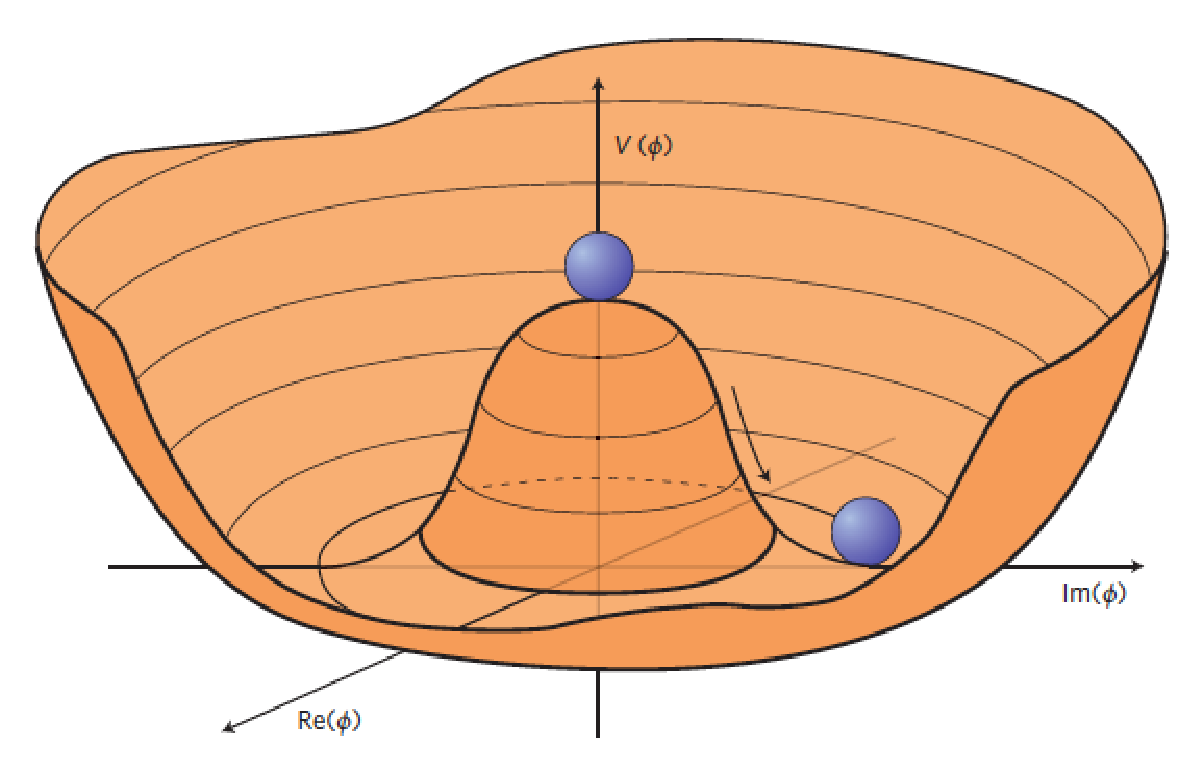
\includegraphics[width=0.75\linewidth]{figures/theory/higgspotential.eps}
\caption{The value of the Higgs potential, $V(\Phi)$ as a function of $\Phi$, for the case that $\mu^2 < 0$ \cite{Ellis:1638469}.}
\label{fig:higgspotential}
\end{figure}

The significant feature of this potential is that its minimum does not occur for a value of $\Phi = 0$. Instead, it is minimized when $|\Phi^\dagger \Phi| = -\mu^2/\lambda$. This means that in its ground state, the Higgs field takes on a non-zero value - referred to as a vacuum expectation value (VEV). So while the Higgs potential is globally symmetric, about the minimum this symmetry is broken. Since the minimum is determined only by $\Phi^\dagger \Phi$, there is some ambiguity in the particular definition of the VEV, but it is generally represented in the unitary gauge as 

\begin{equation}
  \label{eq:VEV}
  \left\langle\Phi\right\rangle = \frac{1}{\sqrt{2}}
  \begin{pmatrix}                                                                                                                               
    0 \\                                                                                                                                   
    v \\                                                                                                                                   
  \end{pmatrix}                                                                                                                       
\end{equation}

The full value of $\Phi$ can be written as 

\begin{equation}                                                                                                                                
  \label{eq:HandV}                                                                                                                                  \left\langle\Phi\right\rangle = \frac{1}{\sqrt{2}}                                                                     
  \begin{pmatrix}                                                                                                                               
    0 \\                                                                                                                   
    v + H\\                                               
  \end{pmatrix}                                                                                                                        
\end{equation}

with $v$ being the value of the VEV, and $H$ being the real value of the scalar field. 

%%%%%%%%%%%%%%%%%%%%%%%%%%%%%%%%%%%%%%%%%%%%%%%%%%%%%%%%%%%%%%%
\subsubsection{Electroweak Symmetry Breaking}
\label{sec:EWKbreaking}

The Electroweak (EWK) interaction is described in the SM by a $SU(2)_L\bigotimes U(1)_Y$ gauge theory. This theory predicts three $SU(2)_L$ gauge boson, $W^1_\mu$, $W^2_\mu$, $W^3_\mu$, and a single $U(1)_Y$ gauge boson, $B_\mu$. The couplings of these bosons to the Higgs field show up in the kinetic terms of the scalar field $\Phi$ in the Lagrangian:

\begin{equation}
  \label{eq:Lphi}
  (D_\mu\Phi)^\dagger(D^\mu\Phi) = |(\partial_\mu - \frac{ig}{2}W^a_\mu\sigma^a - \frac{ig'}{2}B_\mu Y)\phi|^2
\end{equation}

Here $D_\mu$ represents the covariant derivative required to preserve gauge invariance, $g$ and $g'$ represent coupling constant of the gauge bosons, $\sigma^a$ denotes the Pauli matrices of $SU(2)$, and $Y$ represents the hypercharge of $U(1)$. The terms in this interaction which contribute to the masses of the gauge bosons can be written as:

\begin{equation}
  \label{eq:LVEV}
  \frac{1}{2}(0,v)(\frac{g}{2}W^a_\mu\sigma^a - \frac{g'}{2}B_\mu)^2
  \begin{pmatrix}                                                                                                                               
    0 \\                                                                                                                                        
    v \\                                                                                                                                        
  \end{pmatrix}
\end{equation}

Expanding these terms into the mass eigenstates of the electroweak interaction yields four physical gauge bosons, two charged and two neutral, which are linear combinations of the fields $W^1_\mu$, $W^2_\mu$, $W^3_\mu$, and $B_\mu$:

\begin{equation}
\begin{gathered}
  \label{eq:EWKfields}
  W^\pm_\mu = \frac{1}{\sqrt{2}}(W^1_\mu \pm i W^2_\mu) \\
  Z^\mu = \frac{1}{\sqrt(g^2+g'^2)}(-g'B_\mu + gW^3_\mu) \\
  A^\mu = \frac{1}{\sqrt(g^2+g'^2)}(gB_\mu + g'W^3_\mu) \\
\end{gathered}
\end{equation}

And the masses of these fields are given by:

\begin{equation}
\begin{gathered}
  \label{eq:EWKmasses}
  M^2_W = \frac{1}{4}g^2v^2 \\
  M^2_Z = \frac{1}{4}(g^2+g'^2)v^2 \\
  M^2_A = 0 \\
\end{gathered}
\end{equation}

This produces exactly the particles we observe - three massive gauge bosons and a single massless photon. The massless photon represents the portion of the gauge symmetry, a single $U(1)$ of the electromagnetic force, that remains unbroken by the VEV.

Interactions with the Higgs field also lead to the generation of the fermion masses, which in the Lagrangian take the form:

\begin{equation}
  \label{eq:Lfermion}
  y_f (\bar{\psi}_{f,L}\phi \psi_{f,R} + \bar{\psi}_{f,R} \phi^\dagger \psi_{f,L})
\end{equation}

Here $f$ corresponds to each of the fermion flavor, and $y_f$ are matrices containing the Yukawa couplings between the Higgs field and the fermions. After symmetry breaking has occured and $\phi$ has taken on the value of the VEV as written in equation \ref{eq:VEV}, the mass terms of the fermions become $\lambda_\psi v$. Written this way, the fermion masses are proportional to their Yukawa couplings to the VEV, with masses 

\begin{equation}
\label{eq:fMass}
  m_f = y_f\frac{v}{\sqrt{2}}
\end{equation}

Based on the equation \ref{eq:HandV}, an additional mass term arises from the potential $V(\Phi)$. This term can be understood as an excitation of the Higgs field, a scalar boson with mass $m_H = 2\lambda v^2$. This is the Higgs boson, which comes about as a natural prediction of electroweak symmetry breaking. 

The fermions' Yakawa couplings to the VEV take the same form as the fermionss coupling to the Higgs boson. Therefore, the strength of a fermion's interaction with the Higgs is directly proportional to its mass. We now have a model that predicts a Higgs boson with mass $m^2_H = 2\lambda v^2$, which interacts with the fermions with coupling strength $y_f$. Because $\lambda$ and $y_f$ are free parameters of the theory, the mass of the Higgs boson and its interactions with the fermions must be measured experimentally. 

%%%%%%%%%%%%%%%%%%%%%%%%%%%%%%%%%%%%%%%%%%%%%%%%%%%%%%%%%%%%%%%

\subsection{WZ + Heavy Flavor Production}
\label{sec:WZ_theory}

Part \ref{part:wz} is dedicated to a measurement of WZ produced in association with a heavy flavor jet - namely, a charm or b-jet - in the fully leptonic channel. In the instance that both the W and Z bosons decay leptonically, this process produces a final state similar to $t\bar{t}H$, as discussed in section \ref{sec:ttH_theory}, making it an irreducible background for that analysis, and any analysis that includes multiple leptons and b-tagged jets in the final state more broadly.

\begin{figure}[H]
  \centering
  \includegraphics[width=0.35\linewidth]{figures/wz_3l.png}%                                                                 
  \includegraphics[width=0.35\linewidth]{figures/wz_3l_c.png}%                                                               
  \includegraphics[width=0.29\linewidth]{figures/wz_bbar.JPG}
  \caption{Example Feynman diagrams of WZ + heavy flavor production}
  \label{fig:wz_feynman}
\end{figure}

The b-jets produced in this process can be thought of in two different ways: either as originating from the quark ``sea'' of the initial state hadrons, or as the result of a gluon from one the colliding protons splitting into $b\bar{b}$ pairs. However, the heavy flavor contribution to the parton distribution function (PDF) of the proton is uncertain, and simulations of this process disagree depending on which of these two approaches one considers. Regardless of the modelling approach taken, the gluon splitting involved involved in producing the b-quark involves complex QCD calculations that introduce large uncertainties. The same can be said - though to a lesser degree - for charm. This makes WZ + heavy flavor difficult to accurately simulate, and introduces a large uncertainty for any analysis which includes it as a background, motivating a measurement of this process.

This measurement uses 139 $fb^{-1}$ of data collected at a center-of-mass energy of 13 TeV to verify the prediction made the Sherpa Monte Carlo generator \cite{sherpa} in simulating WZ + heavy flavor production.

%%%%%%%%%%%%%%%%%%%%%%%%%%%%%%%%%%%%%%%%%%%%%%%%%%%%%%%%%%%%%%%

\subsection{$t\bar{t}H$ Production}
\label{sec:ttH_theory}

While the SM has been tested to great precision, particularly at the LHC, it is generally accepted that it is only valid up to a certain energy scale. It is assumed that above a certain energy, at the scale where something like a Grand Unified Theory (GUT) or quantum gravity become relevant, the SM will not be applicable. Further, there are several experimental observations that the SM fails to explain. For example, the SM predicts neutrinos to be massless, despite experimental observation to the contrary, and fails to explain the observation of dark matter and dark energy.

Another example, revelant to the Higgs sector, is known as the hierarchy problem: large quantum corrections to the Higgs mass from loop diagrams, such as those shown in Figure \ref{fig:hierarchyDiagram}, are many orders of magnitude larger than the Higgs mass itself. The observed value of the Higgs mass therefore requires extremely precise cancellation between these corrections and the bare mass of the Higgs, a cancellation which seems unnatural and suggests something missing in our theoretical picture.

\begin{figure}[H]
\centering
   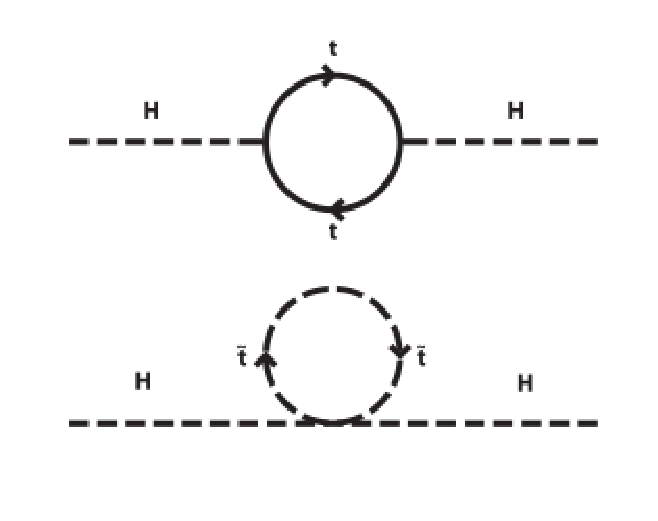
\includegraphics[width=0.5\linewidth]{figures/theory/hierarchyDiagram.eps}
\caption{Above diagram is the leading order correction to the Higgs mass via a top quark loop. Below is a stop squark loop, coming from a supersymmetric extension of the SM which, while not the focus of this paper, is an example of a process that could provide cancellation of the top diagram.}
\label{fig:hierarchyDiagram}
\end{figure}

The strength of a fermion's interaction with the Higgs, given by its Yakawa coupling, is proportionate to its mass. The top quark - as the heaviest known particle - has the strongest interaction, making this interaction particularly interesting to study. While several processes involve interactions between the Higgs and the top, some Higgs production modes include the top interaction only as a part of a loop diagram, such as the gluon-gluon fusion diagram shown in Figure \ref{fig:Hgg}. This process therefore only allows for an indirect probe of the Higgs-top Yakawa coupling, as the flavor of the quark in this diagram is not unique, and can contain other particles.

\begin{figure}[H]
\centering                                                                                                                
   \includegraphics[width=0.5\linewidth]{figures/theory/Hgg.JPG}
\caption{Diagram of a Higgs boson produced via gluon-gluon fusion.}
\label{fig:Hgg}
\end{figure}

Studying the Higgs produced in association with top quark pairs, $t\bar{t}H$, allows this interaction to be measured directly. This process, as shown in Figure \ref{fig:ttH_diagram}, involves a direct coupling between the Higgs and the top, which can be identified by the top quark pair in the final state.

\begin{figure}[H]
\centering
   \includegraphics[width=0.6\linewidth]{figures/theory/ttH_diagram.JPG}
\caption{Diagram of a Higgs boson produced in association with a pair of top quarks.}                         
\label{fig:ttH_diagram}                                                                                    
\end{figure}

The Higgs boson, as well as the top quarks, have very short lifetimes - on the order of $10^{-22}$ s and $10^{-25}$ s respectively - meaning they can only be observed via their decay products. Measuring this process is therefore a matter of identifying events with final states consistent with $t\bar{t}H$ production. 

Studies of $t\bar{t}H$ production have been reported by the ATLAS collaboration for $H\rightarrow b\bar{b}$, $H\rightarrow \gamma\gamma$ and multilepton (encompassing $H\rightarrow W^+W^-$, $H\rightarrow ZZ$ and $H\rightarrow \tau^-\tau^+$, with $H\rightarrow ZZ\rightarrow 4l$ as a separate analysis) decay modes. In multilepton final states, at least one of the light leptons, meaning either muons or electrons, originate from the Higgs decay, with other leptons originating from the decay of the top quarks. The channels targeted by this analysis - with 2 same-sign or three leptons in the final state - both involve the Higgs decaying to intermediate W bosons, $H\rightarrow W^+W^-$. The W bosons can decay either to a single lepton and a neutrino, $W\rightarrow l\nu$, providing the source for light leptons, or hadronically into two quarks. The top quarks effectively always decay to a W boson and a b-quark. The W bosons from the top quark decays provide an additional source for final state leptons in $t\bar{t}H$ events.

While the branching ratio of $H\rightarrow W^+W^-$ is smaller than $H \rightarrow b \bar{b}$ (see Table \ref{tab:H_BR}), it produces a clearer signal, as $H \rightarrow b \bar{b}$ suffers from large $t\bar{t}$ backgrounds. On the other hand, $H\rightarrow \gamma\gamma$ produces the most easily identifiable signal, but has a much smaller branching ratio than $H\rightarrow W^+W^-$. Therefore, compared with other final states of $t\bar{t}H$, the $t\bar{t}H-ML$ channel is an attractive candidate for study, as it involves a good balance between statistical power and identifiability. 

\begin{table}[H]
\centering
\begin{tabular}{lc}
\hline\hline
Decay Mode & Branching Ratio (\%) \\
\hline
$H \rightarrow b \bar{b}$ & 58.2 \\
$H\rightarrow WW^*$ & 21.4 \\
$H\rightarrow gg$ & 8.19 \\
$H\rightarrow \tau\tau$ & 6.27 \\
$H\rightarrow c\bar{c}$ & 2.89 \\
$H\rightarrow ZZ^*$ & 2.62 \\
$H\rightarrow \gamma\gamma$ & 0.227 \\
\hline
\end{tabular}
\label{tab:H_BR}
\caption{Summary of the predominant SM Higgs ($m_H = 125$ GeV) branching ratios. Particles with a star imply off-shell decays.}
\end{table} 

Searches for $t\bar{t}H$ production typically target a measurement of the signal strength parameter, $\mu_{t\bar{t}H}$, which measures the ratio of the observed cross-section and the expected cross-section according to the SM.

\begin{equation}
        \mu_{t\bar{t}H} = \frac{\sigma^{obs.}_{t\bar{t}H}}{\sigma^{SM}_{t\bar{t}H}}
\end{equation}

$t\bar{t}H$ production was observed by ATLAS using up to 79.8 $fb^{-1}$ of data collected at $\sqrt{s}$ = 13 TeV, based on a combination of five Higgs decay modes: $b\bar{b}$, $WW^*$, $\tau^{-}\tau^{+}$, $\gamma\gamma$, and $ZZ^*$ \cite{Higgs_combo}. A significance of $5.8\sigma$ was observed, compared to a $4.9\sigma$ expected significance. Since then, two analyses have published updated results ($H\rightarrow \gamma\gamma$ and $H\rightarrow ZZ^*\rightarrow 4l$) with the full Run 2 dataset, representing 139 $fb^{-1}$. Studies are still ongoing in the remaining channels.

The CMS collaboration has performed similar searched for $t\bar{t}H$, acheiving an observed (expected) significance of 5.2$\sigma$ (4.2$\sigma$) across each of the Higgs decay modes using data collected from 2011-2017 with center of mass energies of 7, 8, and 13 TeV \cite{PhysRevLett.120.231801}. 

%%%%%%%%%%%%%%%%%%%%%%%%%%%%%%%%%%%%%%%%%%%%%%%%%%%%%%%%%%%%%%%

\subsection{Differential Measurements of $t\bar{t}H$}
\label{sec:bsm}

While $t\bar{t}H$ has been observed by both the ATLAS \cite{ttH_paper} and CMS \cite{Sirunyan_2018} collaborations, these analyses have focused on measuring the overall rate of $t\bar{t}H$ production. There are several theories of physics Beyond the Standard Model (BSM), however, that could affect the kinematics of $t\bar{t}H$ production without significantly altering its overall rate \cite{Dumont_2013}.

An Effective Field Theory approach can be used to model the low energy effects of new, high energy physics, by paramaterizing BSM effects as higher dimensional operators. These additional operators can then be added to the SM Lagrangian to write an effective Lagrangian that accounts for the effects of these higher energy physics. The lowest order of these that could contribute to Higgs-top coupings are dimension-six, as represented in Equation \ref{eq:dim6}.

\begin{equation}
\label{eq:dim6}
\mathcal{L}_{eff} = \mathcal{L}_{SM} + \frac{f}{\Lambda}\mathcal{O}^6
\end{equation}

Here $\Lambda$ represents the energy scale of the new physics, $f$ is a Wilson coefficient which represents the strength of the effective coupling, and $\mathcal{O}$ is the operator. An experimental observation of any non-zero value of $f$ would be a sign of BSM physics.

The addition of these operators can be shown to modify the transverse momentum ($p_T$) spectrum of the Higgs Boson in Higg-top interactions, without significantly affecting the overall rate of $t\bar{t}H$ production \cite{Banerjee_2014}. The possible impact of these higher order effects on the Higgs $p_T$ spectrum are shown in Figure \ref{fig:eft_pt}. Here the additional operators include an effective quartic coupling between the gluon, Higgs, and a pair of top quarks, the strength of which is represented by $C_{ght}$, and a loop-induced interaction between the gluon and Higgs, $C_{GH}$. In this example the parameters are chosen such that the overall rate of $t\bar{t}H$ production remains the same as the Standard Model prediction.

\begin{figure}[H]
\centering
   \includegraphics[width=0.5\linewidth]{figures/theory/higgs_pt.PNG}
\caption{The momentum spectrum of the Higgs boson produced via top-quarks with (red) and without (blue) the presence of a particular choice of dimension-six operator.  \cite{Banerjee_2014}.}
\label{fig:eft_pt}
\end{figure}

Here the additional operators include an effective quartic coupling between the gluon, Higgs, and a pair of top quarks, shown in Equation \ref{eq:gtth}, the strength of which is represented by $C_{ght}$. $C_{GH}$ is the strength of a loop-induced interaction between the gluon and Higgs \ref{eq:gh}. In this example the values of these couplings are chosen such that the overall rate of $t\bar{t}H$ production remains the same as the Standard Model prediction.

\begin{equation}
\label{eq:gtth}
(\tilde{q}\sigma^{\mu\nu}T^At)\tilde{\phi}G^A_{\mu\nu}
\end{equation}


\begin{equation}
\label{eq:gh}
(\phi^\dagger\phi)G^A_{\mu\nu}G^{A\mu\nu}
\end{equation}


This provides a clear, physics observable that could be used to search for evidence of BSM physics using data collected at the LHC. Reconstructing the momentum spectrum of the Higgs in $t\bar{t}H$ events therefore provides a means to search for new physics in the Higgs sector.

Reconstructing the Higgs is a particular challenge in the multilepton channels of $t\bar{t}H$, due to an ambiguity arising from multiple sources of missing energy. In the $H\rightarrow \gamma\gamma$ channel, the kinematics of the Higgs can be fully reconstructed from the two photons. The same is true of $H\rightarrow b\bar{b}$, though with the additional challenge of identifying which two of the four b-quarks in the final state originated from the Higgs. By contrast, the two channels ($2lSS$ and $3l$) targeted by this analysis include at least one neutrino originating from the Higgs decay. 

\begin{figure}[H]
    \centering
    \subfigure[]{\includegraphics[width=.43\linewidth]{theory/ttH-2lSS.JPG}}%                             
    \subfigure[]{\includegraphics[width=.43\linewidth]{theory/ttH-3l.JPG}}%                                
    \caption{Feynman diagrams of $t\bar{t}H$ production with (a) two same-sign leptons and (b) three leptons in the final state.}
    \label{fig:ttH-2lSS-3l}
\end{figure}

Neutrinos are not detected by ATLAS; instead, their presence is inferred from missing transverse energy in the detector, $E^T_{miss}$. The two channels targeted here include not just a neutrino from the Higgs decay, but at least one additional neutrino from the decay of the top-quarks. This makes disentangling the contribution of the Higgs decay to $E^T_{miss}$, and thereby fully reconstructing the Higgs, impossible. This challenge motivates the use of more sophisticated machine learning techniques when attempting to perform differential measurements of the Higgs $p_T$ spectrum in the multi-lepton channels of $t\bar{t}H$. 

Chapter \ref{part:analysis} provides exploratory studies on the feasibility of differential measurements of $t\bar{t}H-ML$, specifically targeting events with two same-sign leptons ($2lSS$) or three leptons ($3l$) in the final state. This includes $H \rightarrow W^+W^-$ events, where at least one of the W bosons decays leptonically. The techniques used to reconstruct the Higgs transverse momentum spectrum are explained, and preliminary results are shown for data collected by ATLAS from 2015-2017, with projected results shown for the full 2015-2018 dataset.

%%%%%%%%%%%%%%%%%%%%%%%%%%%%%%%%%%%%%%%%%%%%%%%%%%%%%%%%%%%%%%% 


\index{The Standard Model and the Higgs Boson@\emph{The Standard Model and the Higgs Boson}}% 
%------------------------------------------------------------------------------

%\section{Effective Field Theory in $t\bar{t}H$ Production}
%\label{sec:eft}
%Higher dimension operators are a common way to paramaterize the effects of physics at very high energies into

%------------------------------------------------------------------------------

%-------------------------------------------------------------------------------
%-------------------------------------------------------------------------------

\chapter{The LHC and the ATLAS Detector}
\label{part:lhcAtlas}

%-------------------------------------------------------------------------------

\section{The LHC}
\label{sec:lhc}
\index{The LHC@\emph{The LHC}}
The Large Hadron Collider (LHC) is a particle accelerator consisting of a 27 km ring, designed to collide protons at high energy. Located outside of Geneva, Switzerland and buried about 100 m undergound, it consists of a ring of superconducting magnets which are used to accelerate opposing beams of protons - or lead ions - which collide at the center of one of the various detectors located around the LHC ring which record the result of these collisions. These detectors include two general purpose detectors, ATLAS and CMS, which are designed to make precision measurements of a broad range of physics phenomenon, and two more specialized experiments, LHCb and ALICE, which are optimized to study b-quarks and heavy-ion physics, respectively.

The LHC first began running in 2009 at a proton-proton center of mass energy of $\sqrt{s} = 2$ TeV. This was increased to 7 TeV in 2010-2011, and again increased to 8 TeV in 2012. The period from 2009 to 2012 is known as Run 1, and data collected during this period was used in discovering the Higgs Boson. The LHC began running again in 2015, and collected data at an increased energy of $\sqrt{s} = 13$ TeV until 2018, a period referred to as Run 2. 

Protons are fed into the LHC via a chain of accelerators, which accelerate the protons to higher and higher energies until they are injected into the main ring. This process is summarized in figure \ref{fig:AccChain}. Protons extracted from a tank of hydrogen are fed into a linear accelerator, LINAC2, where they reach an energy of 50 MeV. From there, they enter a series of three separate circular accelerators, before being injected into the main accelerator ring at an energy of 450 GeV. Within the main ring protons are seperated into two seperate beams moving in opposite directions, and their energy is increased to their full collision energy. Radiofrequency cavities are used to accelerate these particles and sort them into bunches. From 2015-2018, these bunches consisted of around 100 billion protons each with an energy of 6.5 TeV per proton, which collided at a rate of 40 MHz, or every 25 ns. 

\begin{figure}[H]
\centering
   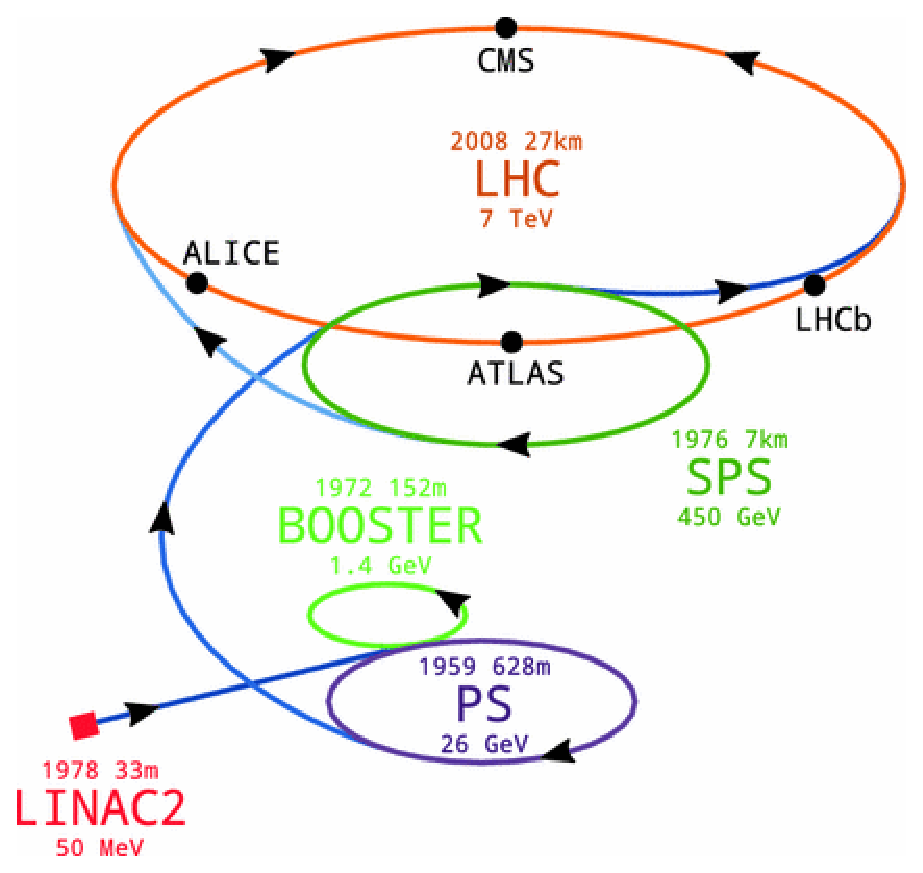
\includegraphics[width=0.7\linewidth]{figures/lhc/AccChain.eps}
\caption{A summary of the accelerator chain used to feed protons into the LHC \cite{accChainFig}.}
\label{fig:AccChain}
\end{figure}

Because these proton bunches consist of a large number of particles, each bunch crossing consists of not just one, but several direct proton-proton collisions. The additional interactions that occur in each bunch crossing, $\mu$, is known as pileup. During Run 2, the average pileup was around $\left\langle\mu\right\rangle$ = 35, with values typically ranging between 10 and 70.

The amount of data collected by the LHC is measured in terms of luminosity, which is the ratio of the number of events detected per unit time, $\frac{dN}{dt}$, and the interaction cross-section, $\sigma$. 

\begin{equation}                                                                                                                                
        \label{eq:lumiDef}                                                                                                                      
        \mathcal{L} = \frac{1}{\sigma}\frac{dN}{dt}
\end{equation}

The design luminosity of the LHC is $10^{34}\ cm^{-2}s^{-1}$, however the LHC has acheived a luminosity of over $2\times 10^{34}\ cm^{-2}s^{-1}$. The total luminosity is then this instantaneous luminosity integrated over time.

\begin{equation}
        \label{eq:intLumi}      
        \mathcal{L}_{int} = \int\mathcal{L}dt
\end{equation}

The integrated luminosity collected by the ATLAS detector as of the end of 2018 is around 140 $fb^{-1}$, exceeding the expected integrated luminosity of 100 $fb^{-1}$. This luminosity is obtained using the LUCID-2 detector \cite{LUCID2} for the primary luminosity measurements using the van der Meer (vdM) method. \cite{Balagura_2021}. This involves varying the location of one of the proton beams and observing how the collision rate is effected.
                                            
                                         


%------------------------------------------------------------------------------

\section{The ATLAS Detector}
\label{sec:atlas}
ATLAS (a not terribly natural acronym for ``A Toroidal LHC Apparatus'') is a general purpose detector designed to maximize the detection efficiency of all physics objects, including leptons, jets, and photons. This means it is capable of measuring all SM particles, with the exception of neutrinos, the presence of which can be inferred based on missing transverse momentum. The detector measures 44 m long, and 25 m tall. 

The ATLAS detector consists of multiple layers, each of which serves a different purpose in reconstructing collisions. At the very center of the detector is the interaction point where the proton beams of the LHC collide. 

\begin{figure}[H]
\centering
   \includegraphics[width=0.75\linewidth]{figures/lhc/ATLASdiagram.eps}
\caption{Cutaway view of the ATLAS detector, with labels of its major components \cite{ATLAS_figure}.}
\label{fig:ATLAS}
\end{figure}

\subsection{Inner Detector}
\label{sec:innerDetector}

\begin{figure}[H]
\centering
   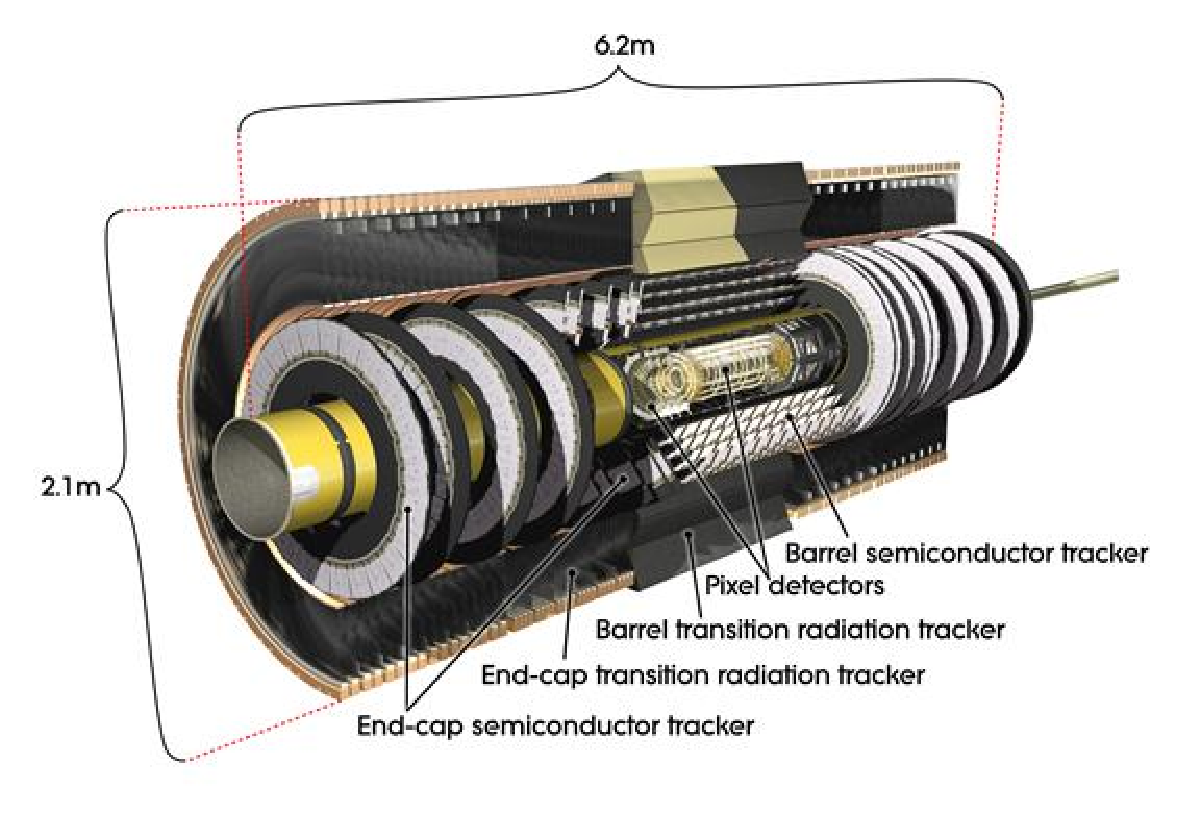
\includegraphics[width=0.75\linewidth]{figures/lhc/InnerDetector.eps}
\caption{Cutaway view of the Inner Detector \cite{caloFig}.}
\label{fig:innerDect}
\end{figure}

Just surrounding the interaction point is the Inner Detector, designed to track the path of charged particles moving through the detector. An inner solenoid surrounding the Innder Detector is used to produces a magnetic field of 2 T. This large magnetic field causes the path of charged particles moving through the Inner Detector to bend. Because this magnetic field is uniform and well known, it can be used in conjunction with the curvature of a particles path to measure its charge and momentum.

The Inner Detector consists of three components - the Pixel Detector, the Semi-Conductor Tracker (SCT), and the Transition Radiation Tracker (TRT). The Pixel Detector is the innermost of these, beginning just 33.25 mm away from the beam line. It consists of three silicon layers along the barrel, as well as three endcap layers, covering a range of $|\eta|$ < 2.5. 

The Semiconductor Tracker (SCT) is similar to the Pixel detector, but uses long strips rather than small pixel to cover a larger spatial area.

\subsection{Calorimeters}
\label{sec:calo}

\begin{figure}[H]
\centering
   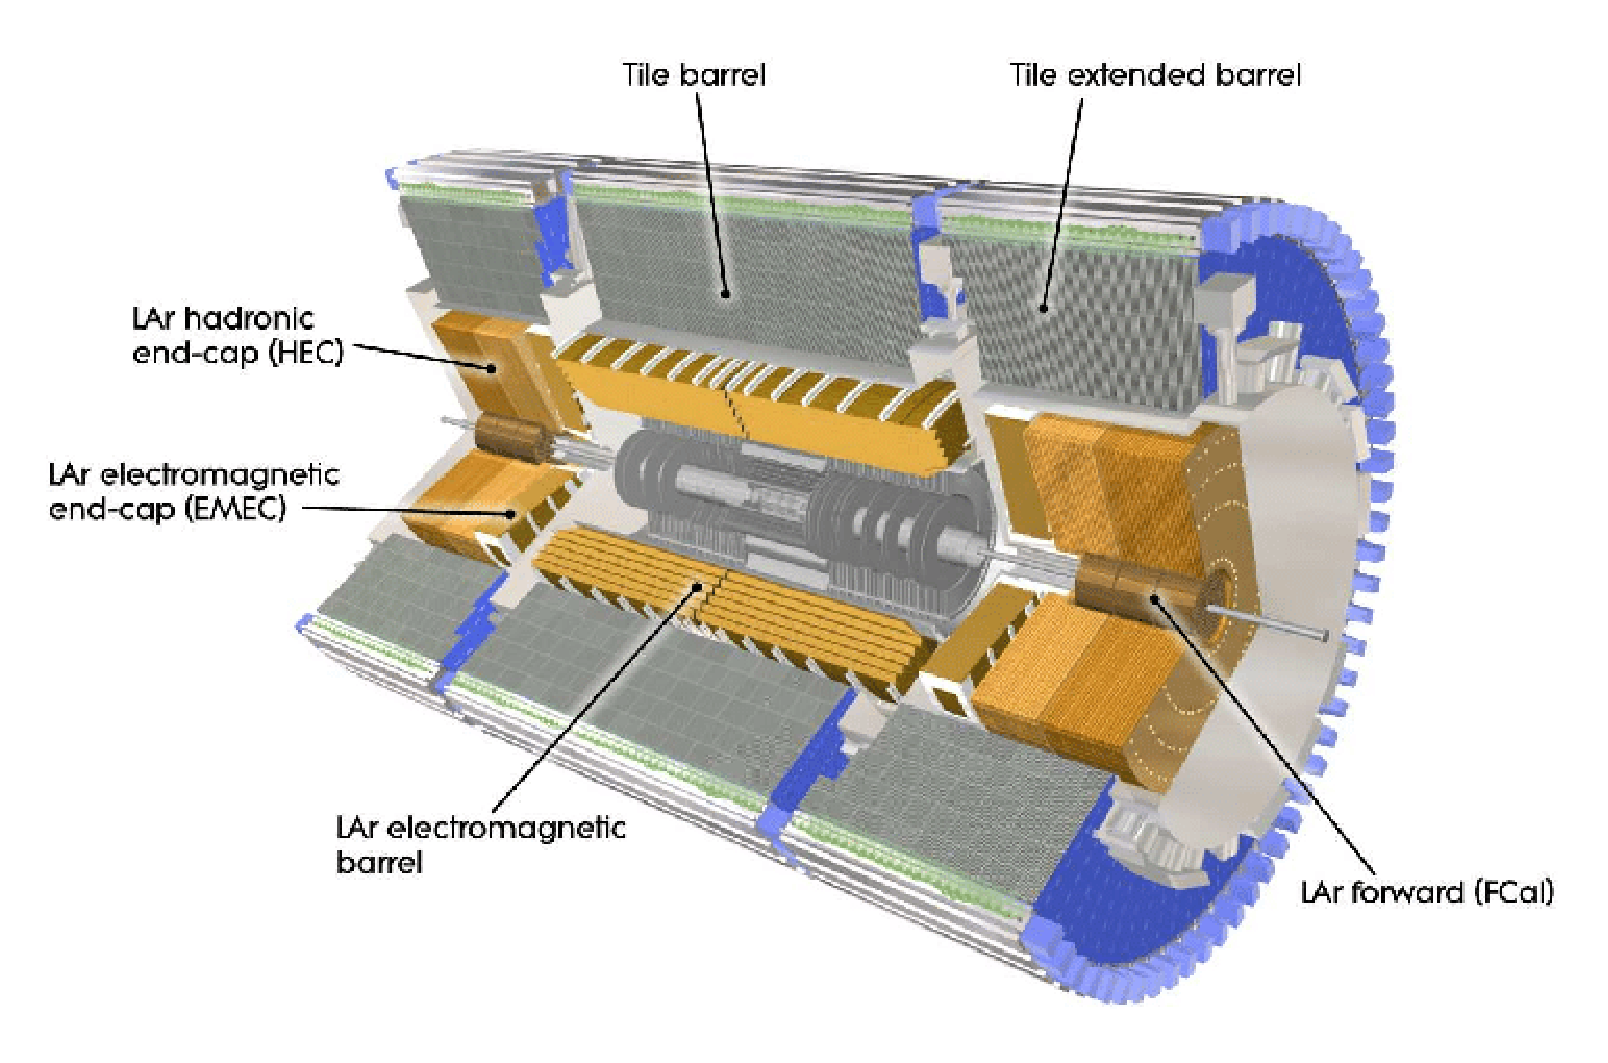
\includegraphics[width=0.9\linewidth]{figures/lhc/calorimeter.eps}
\caption{Cutaway view of the calorimeter system of the ATLAS detector \cite{caloFig}.}
\label{fig:calo}
\end{figure}

Situated outside the Innder Detector are two concentric calorimeters. The inner calorimeter uses liquid argon (LAr) to measure energy of particles the interact electromagnetically, which includes photons and any charged particle. The LAr calorimeter is made of heavy metals, primarily lead and copper, which causes electromagnetically interacting particles to shower, depositing their energy in the detector. The showering of the high energy particles that pass through calorimeter cause the liquid argon to ionize, and the ionized electrons are detected by electronic readouts. The LAr calorimeter consists of around 180,000 readout channels.  

The outer calorimeter measures the energy from particles that pass through the EM calorimeter, and measures the energy of particles that interact via the strong force. This is primarily hadrons. It is composed of steel plates to cause hadronic showering and scintillating tiles as the active material. The signals from the hadronic calorimeter are read out by photomultiplier tubes (PMTs).

\subsection{Muon Spectrometer}
\label{sec:muonSpec}

Because muons are heavier than electrons and photons, and do not interact via the strong force, they generally pass through the detector without being stopped by the calorimeters. The outermost components of the detector are designed specifically to measure the energy and momentum of muons produced in the LHC. The muon spectrometer consists of tracking and triggering system. It extends from the outside of the calormeter system, about a 4.25 m radius from the beam line, to a radius of 11 m. This large detector system is necessary to accurately measure the momentum of muons, which is essential not only for measurements involving the muons themselves, but also to accurately estimate the missing energy in each event.

Two large toroidal magnets within the muon system generate a large magnetic field which covers an area 26 m long with a radius of 10 m. Because the area covered by this magnet system is so large, a uniform magnetic field like the one produced in the Inner Detector is impractical. Instead, the magnetic field that exists in the muon spectrometer ranges between 2 T and 8 T, and is much less uniform. The path of the muons passing through the spectrometer is bent by this field, allowing their charge to be determined. 

1200 tracking chambers are placed in the muon system in order to precisely measure the tracks of muons with high spatial resolution.

%\subsection{Forward Detector}
%\label{sec:forwardDet}

\subsection{Trigger System}
\label{sec:trigger}

Because of the high collision rate and large amount of data collected by the various subdetectors, ATLAS produces far more data than can actually be stored. Each event produces around 25 Mb of raw data, which multiplied by the bunch crossing rate of 40 MHz, comes out to around a petabyte of data every second. The information from every event cannot practically be stored, therefore a sophisticated trigger system is employed in real time to determine whether events are sufficiently interesting to be worth storing.

The trigger system in ATLAS involves multiple levels, each of which select out which events move on to the next level of scrutiny. The level-1 trigger uses hardware information from the calorimeters and muon spectrometer to select events that contain candidates for particles commonly used in analysis, such as energetic leptons and jets. The level-1 trigger reduces the rate of events from 40 MHz to around 100 kHz. 

Events that pass the level-1 trigger move to the High-Level Trigger (HLT). The HLT takes place outside of the detector in software, and looks for properties such as a large amount of missing transverse energy, well defined leptons, and multiple high energy jets. Events that pass the HLT are stored and used for analysis. Because the specifics of the HLT are determined by software rather than hardware, the thresholds can be changed throughout the run of the detector in response to run conditions such as changes to pilup and luminosity. After the HLT is applied, the event rate is reduced to around 1000 per second, which are recorded for analysis.


%------------------------------------------------------------------------------- 
%-------------------------------------------------------------------------------                                             
 
\chapter{Measurement of WZ + Heavy Flavor}                                                                                    
\label{part:wz}

%------------------------------------------------------------------------------

%-------------------------------------------------------------------------------                                             
\section{Introduction}                                                                                                      
\label{sec:intro}                                                                                                           
Since the discovery of a Higgs boson compatable with the Standard Model (SM) in 2012 \cite{HIGG-2011-02}, its interactions with other particles have been studied using proton-proton collision data produced by the Large Hadron Collider (LHC). The strongest of these interactions is the coupling of the Higgs to the top quark, making the Yukawa coupling between these two particles of particular interest for study.

These interactions can be measured directly by studying the production of a Higgs Boson in association with a pair of Top Quarks ($t\bar{t}H$). While this process has been observed by both the ATLAS and CMS collaborations, these analyses have focused on measuring the overall rate of $t\bar{t}H$ production. There are several theories of physics Beyond the Standard Model (BSM), however, that would affect the kinematics involved in $t\bar{t}H$ production without altering its overall rate \cite{Dumont_2013}.  

An Effective Field Theory approach can be used to model the low energy effects of new, high energy physics, by paramaterizing BSM effects as dimension-six operators. The addition of these operators can be shown to modify the transverse momentum ($p_T$) spectrum of the Higgs Boson \cite{Banerjee_2014}. Therefore, reconstructing the momentum spectrum of the Higgs provides a means to observe new physics in the Higgs sector.  

This note reports on the feasability of performing differential measurements in $t\bar{t}H$ events with multiple leptons in the final state, using Monte Carlo (MC) simulations scaled to 139 $fb^{-1}$ at an energy $\sqrt{s} = 13$ TeV. Events are separated into channels based on the number of light leptons (electrons and muons) in the final state - either two same-sign leptons ($2lSS$), or three leptons ($3l$), where the $3l$ channel is split into two based on the decay of the Higgs.

The presence of multiple neutrinos in the final state of the multilepton channels introduces an ambiguity that prevents the Higgs from being fully recontructed. This motivates the use of sophisticated machine learning techniques to better predict the Higgs \pt spectrum for these events. A deep neural network is used to identify which objects originate from the decay of the Higgs, and reconstruct the momentum of the Higgs Boson in each event. This spectrum is fit to data in the three decay channels considered in order to extract normalization factors on $t\bar{t}H$ produced with high ($>150$ GeV) and low ($<150$ GeV) Higgs.

This note is organized as follows: The dataset and Monte Carlo (MC) simulations used in the analysis is outlined in Section \ref{sec:dataMC}. Section \ref{sec:objReco} describes the identification and reconstruction of the various physics objects. The models used to reconstruct the momentum spectrum of the Higgs is discussed in Section \ref{sec:mva}. The selection and categorisation of events comprises Section \ref{sec:signal_region}, and the theoritical and experimental systematic uncertainties considered are described in Section \ref{sec:sys}. Finally, the results of the study are summarized in Section \ref{sec:results}.
                                                                                                      
%-------------------------------------------------------------------------------

%-------------------------------------------------------------------------------                                             
\section{Data and Monte Carlo Samples}
\label{sec:data}
\input{wz_sections/MC}
%-------------------------------------------------------------------------------                                             
 
%-------------------------------------------------------------------------------                                             
\section{Object Reconstruction}
\label{sec:obj}
\input{wz_sections/reco}
%-------------------------------------------------------------------------------                                             
 
%-------------------------------------------------------------------------------                                             
\section{Event Selection and Signal Region Definitions}
\label{sec:evt_selection}
\input{wz_sections/evtSel}
%-------------------------------------------------------------------------------                                             
 
%-------------------------------------------------------------------------------                                             
\section{tZ Separation Multivariate Analysis}
\label{sec:tZ_bdt}
\input{wz_sections/tZ}
%-------------------------------------------------------------------------------

%-------------------------------------------------------------------------------                                             
\section{Systematic Uncertainties}
\label{sec:sys}
\input{wz_sections/sys}                                                                              
%-------------------------------------------------------------------------------                                             
                                                                                                                             
%-------------------------------------------------------------------------------                                           
\section{Results}
\label{sec:results}                                                                                                          
\input{wz_sections/truthJetResults}
%-------------------------------------------------------------------------------

%------------------------------------------------------------------------------- 
\section{Conclusion}
\label{sec:conclusion}

A measurement of $WZ$ + heavy flavor is performed using 140 $fb^{-1}$ of $\sqrt{s} = 13$ TeV proton-proton collision data collected by the ATLAS detector at the LHC. The expected cross-section of WZ + $b$ with 1-jet is $1.74^{+0.82}_{-0.75}(stat)^{+0.53}_{-0.48}(sys)$ fb, and $14.6 \pm 2.5 (stat) \pm 2.3 (sys)$ fb for WZ + $c$, with a correlation of -0.22 between them. An expected significance of 2.0 is observed for WZ + $b$ in this region.

For the 2-jet regions, an expected significance of 1.7 is observed for WZ + $b$, with an expected cross-section of $2.5^{+1.3}_{-1.3}(stat)^{+0.95}_{-0.83}(sys)$ fb. For WZ + $c$, a cross-section of $12.7 \pm 3.2 (stat) \pm 2.7 (sys)$ fb is expected for 2-jet events. A correlation of -0.26 is observed for WZ + $b$ and WZ + $c$.

\textbf{This section will be include final results once unblinded.}
%------------------------------------------------------------------------------- 

%-------------------------------------------------------------------------------
%-------------------------------------------------------------------------------

\chapter{Differential Studies of $t\bar{t}H$ Multilepton }
\label{part:analysis}

%-------------------------------------------------------------------------------

\section{Data and Monte Carlo Samples}
\label{sec:dataMC}
This study used data collected by the ATLAS detector over the period from 2015-2018, representing 138.9 $fb^{-1}$ of data at an energy of 13 TeV. 

Several Monte Carlo generators were used to simulate both signal and background processes. For all of these, the effects of the ATLAS detector are simulated in Geant4. 

%-------------------------------------------------------------------------------   

\section{Object Reconstruction}
\label{sec:objReco}

All analysis channels considered in this note share a common object selection for leptons and jets, as well as a shared trigger selection. 

\subsection{Trigger Requirements}

Events are required to be selected by dilepton triggers, as summarized in table \ref{tbl:trigger}.

\begin{table}[h!]
 \begin{center}
   \begin{tabular}{cc}
     \toprule
                  & Dilepton triggers (2015) \\
     \midrule
      $\mu\mu$ (asymm.)          & \verb!HLT_mu18_mu8noL1! \\
      $ee$ (symm.)               & \verb!HLT_2e12_lhloose_L12EM10VH! \\
      $e\mu,\mu e$ ($\sim$symm.) & \verb!HLT_e17_lhloose_mu14! \\
     \bottomrule
                       & Dilepton triggers (2016) \\
     \midrule
      $\mu\mu$ (asymm.)                   & \verb!HLT_mu22_mu8noL1! \\
      $ee$ (symm.)                        & \verb!HLT_2e17_lhvloose_nod0! \\
      $e\mu,\mu e$ ($\sim$symm.)          & \verb!HLT_e17_lhloose_nod0_mu14! \\
     \bottomrule

                  & Dilepton triggers (2017) \\
     \midrule
      $\mu\mu$ (asymm.)                   & \verb!HLT_mu22_mu8noL1! \\
      $ee$ (symm.)                        & \verb!HLT_2e24_lhvloose_nod0! \\
      $e\mu,\mu e$ ($\sim$symm.)          & \verb!HLT_e17_lhloose_nod0_mu14! \\
     \bottomrule
                  & Dilepton triggers (2018) \\
     \midrule
      $\mu\mu$ (asymm.)                   & \verb!HLT_mu22_mu8noL1! \\
      $ee$ (symm.)                        & \verb!HLT_2e24_lhvloose_nod0! \\
      $e\mu,\mu e$ ($\sim$symm.)          & \verb!HLT_e17_lhloose_nod0_mu14! \\
      \bottomrule
   \end{tabular}
   \caption{\label{tbl:trigger} List of lowest $p_{T}$-threshold, un-prescaled dilepton triggers used for 2015-2018 data taking.}
 \end{center}
\end{table}

\subsection{Light Leptons}
\label{subsec:lepSelection}

Electron candidates are reconstructed from energy clusters in the electromagnetic calorimeter that are associated with charged particle tracks reconstructed in the inner detector \cite{ATLAS-CONF-2016-024}.  Electron candidates are required to have $\pt > 10$ GeV and $|\eta_\textrm{cluster}| < 2.47$. Candidates in the transition region between different electromagnetic calorimeter components, $1.37 < |\eta_\textrm{cluster}| < 1.52$, are rejected. A multivariate likelihood discriminant combining shower shape and track information is used to distinguish prompt electrons from nonprompt leptons, such as those originating from hadronic showers. 

To further reduce the non-prompt contribution, the track of each electron is required to originate from the primary vertex; requirements are imposed on the transverse impact parameter significance ($|d_0|/\sigma_{d_0}$) and the longitudinal impact parameter ($|\Delta z_0 \sin \theta_\ell|$), as shown in table \ref{tbl:tightleps}.

Muon candidates are reconstructed by combining inner detector tracks with track segments or full tracks in the muon spectrometer \cite{PERF-2014-05}. Muon candidates are required to have $\pt > 10$~GeV and $|\eta| < 2.5$. All leptons are required to be isolated, and pass a non-prompt BDT selection described in detail in \cite{ttH_paper}.

\subsection{Jets}
\label{subsec:jetSelection}

%UPDATE TO PFLOW
Jets are reconstructed from calibrated topological clusters built from energy deposits in the calorimeters \cite{ATL-PHYS-PUB-2015-015}, using the anti-$k_t$ algorithm with a radius parameter $R=0.4$.  Jets with energy contributions likely arising from noise or detector effects are removed from consideration \cite{ATLAS-CONF-2015-029}, and only jets satisfying $\pt > 25$~GeV and $|\eta| < 2.5$ are used in this analysis.  For jets with $\pt < 60$~GeV and $|\eta| < 2.4$, a jet-track association algorithm is used to confirm that the jet originates from the selected primary vertex, in order to reject jets arising from pileup collisions \cite{PERF-2014-03}. 

\subsection{Missing Transverse Energy}

Because all $t\bar{t}H-ML$ channels considered include multiple neutrinos, missing transverse energy ($E_T^{miss}$) is present in each event. The missing transverse momentum vector is defined as the inverse of the sum of the transverse momenta of all reconstructed physics objects as well as remaining unclustered energy, the latter of which is estimated from low-\pt tracks associated with the primary vertex but not assigned to a hard object \cite{ATL-PHYS-PUB-2015-027}.


%------------------------------------------------------------------------------- 

\section{Higgs Momentum Reconstruction}
\label{sec:mva}
Reconstructing the momentum of the Higgs boson is a particular challenge for channels with leptons in the final state: Because all channels include at least two neutrinos in the final state, the Higgs can never be fully reconstructed. However, the momentum spectrum can be well predicted by a neural network when provided with the four-vectors of the Higgs Boson decay products, as shown in section \ref{sec:truthLevelReco}. With this in mind, a sophisticated approach involving several layers of MVAs is used to reconstruction the Higgs momentum. 

The first layer is a Neural Network designed to select which jets are most likely to be the b-jets that came from the top decay. The kinematics of these jets are fed into the second layer, also a BDT, which is designed to identify the decay products of the Higgs Boson itself. The kinematics of these particles are then fed into a deep neural-network, which predicts the momentum of the Higgs.

\subsection{Truth Level Reconstruction}
\label{sec:truthLevelReco}

Machine Learning algorithms are trained to identify the decay products of the Higgs Boson using MC simulations of $t\bar{t}H$ events. Reconstructed physics objects are matched to truth level particles, in order to identify the parents of these reconstructed objects. 

\subsection{b-jet Identification}
\label{sec:bjetID}

In both the 3l and 2lSS channels, one or b-tagged jet is required. Therefore, for events which have exactly one, or more than two, b-tagged jets, deciding which combination of jets correspond to the top decay

\subsection{Higgs Reconstruction}
\label{sec:higgsID}

Techniques similar to the b-jet identification algorithms are employed to select the decay products of the Higgs. 

\subsection{$p_T$ Prediction}
\label{sec:ptReco}

Once the most probable decay products have been identified, their kinematics are used to reconstruct the momentum spectrum of the Higgs Boson. 

\subsection{3l Decay Mode}
\label{sec:decay3l}

In the 3l channel, there are two possible ways for the Higgs to decay, both involving intermediate W boson pairs: Either both W bosons decay leptonically, in which case the reconstructed decay consists of two leptons (referred as the fully-leptonic 3l channel), or one W decays leptonically and the other hadronically, giving two jets and one lepton in the final state (referred to as the semi-leptonic 3l channel). In order to accurately reconstruct the Higgs, it is necessary to identify which of these decays took place for each 3l event.





%---------------------------------------------------------------------

\section{Signal Region Definitions}
\label{sec:signal_region}
Events are divided into two channels based on the number of leptons in the final state: one with two same-sign leptons, the other with three leptons. The $3l$ channel includes events where both leptons originated from the Higgs boson as well as events where only one of the leptons 

%------------------------------------------------------------------------------------------

\subsection{Pre-MVA Event Selection}
\label{subsec:preMVA}

A preselection is applied to define orthogonal analysis channels based on the number of leptons in each event. For the 2lSS channel, the following presection is used:

\begin{itemize}
  \item Two very tight, same-charge, light leptons with $p_T > 20$ GeV
  \item $>=$4 reconstructed jets, $>=$1 b-tagged jets
  \item No reconstructed tau candidates
\end{itemize}

\begin{figure}[h!]
    \subfigure[]{\includegraphics[width=.29\linewidth]{trexPlots/stat2l_80/Plots/lep_Pt_0.png}}%                        
    \subfigure[]{\includegraphics[width=.29\linewidth]{trexPlots/stat2l_80/Plots/lep_Pt_1.png}}%                     
    \subfigure[]{\includegraphics[width=.29\linewidth]{trexPlots/stat2l_80/Plots/Mll01}}\\
    \subfigure[]{\includegraphics[width=.29\linewidth]{trexPlots/stat2l_80/Plots/nJets.png}}%                       
    \subfigure[]{\includegraphics[width=.29\linewidth]{trexPlots/stat2l_80/Plots/nbJets.png}}%                
    \subfigure[]{\includegraphics[width=.29\linewidth]{trexPlots/stat2l_80/Plots/MET.png}}\\
    \caption{}                           
    \label{fig:presel2lSS}
\end{figure}

For the 3l channel, the following selection is applied:

\begin{itemize}
  \item Three light leptons with total charge $\pm 1$
  \item Same charge leptons are required to be very tight, with $p_T > 20$ GeV
  \item Opposite charge lepton must be loose, with $p_T > 10$ GeV
  \item $>=$2 reconstructed jets, $>=$1 b-tagged jets                                                                        
  \item No reconstructed tau candidates
  \item $|M(l^+l^-)-91.2\textrm{ GeV}| > 10$~\GeV{} for all opposite-charge, same-flavor lepton pairs
\end{itemize}

\begin{figure}[h!]
    \subfigure[]{\includegraphics[width=.29\linewidth]{trexPlots/stat3l_80/Plots/lep_Pt_0.png}}%                             
    \subfigure[]{\includegraphics[width=.29\linewidth]{trexPlots/stat3l_80/Plots/lep_Pt_1.png}}%                      
    \subfigure[]{\includegraphics[width=.29\linewidth]{trexPlots/stat3l_80/Plots/Mll01}}\\                             
    \subfigure[]{\includegraphics[width=.29\linewidth]{trexPlots/stat3l_80/Plots/nJets.png}}%                          
    \subfigure[]{\includegraphics[width=.29\linewidth]{trexPlots/stat3l_80/Plots/nbJets.png}}%                          
    \subfigure[]{\includegraphics[width=.29\linewidth]{trexPlots/stat3l_80/Plots/MET.png}}\\                         
    \caption{}
    \label{fig:presel3l}                                                                                          
\end{figure}

%------------------------------------------------------------------------------------------

\subsection{Event MVA}
\label{subsec:sigBkgMVA}

Separate multi-variate analysis techniques (MVAs) are used in order to distinguish signal events from background for each analysis channel - 2lSS, 3l semi-leptonic, and 3l fully leptonic. In particular, Neural Networks produced with Tensorflow are trained using the kinematics of signal and background events derived from Monte Carlo simulations. Further, because the background composition differs for events with a high reconstructed Higgs $p_T$ compared to events with low reconstructed Higgs $p_T$, separate MVAs are produced for high and low $p_T$ regions.

Output distributions of each MVA are shown in figure \ref{fig:sigBkgScore}. Detailed explanations of each of the models can be found in section \ref{apx:MVA}.

\begin{figure}
  \subfigure[]{\includegraphics[width=.3\linewidth]{trexPlots/xgb_higgsDiff/Plots/xgb_sigBkg_2lHigh.png}}%
  \subfigure[]{\includegraphics[width=.3\linewidth]{trexPlots/xgb_higgsDiff/Plots/xgb_sigBkg_3lSHigh.png}}%
  \subfigure[]{\includegraphics[width=.3\linewidth]{trexPlots/xgb_higgsDiff/Plots/xgb_sigBkg_3lFHigh.png}}\\
  \subfigure[]{\includegraphics[width=.3\linewidth]{trexPlots/xgb_higgsDiff/Plots/xgb_sigBkg_2lLow.png}}%
  \subfigure[]{\includegraphics[width=.3\linewidth]{trexPlots/xgb_higgsDiff/Plots/xgb_sigBkg_3lSLow.png}}%
  \subfigure[]{\includegraphics[width=.3\linewidth]{trexPlots/xgb_higgsDiff/Plots/xgb_sigBkg_3lFLow.png}}
  \label{fig:sigBkgScore}
  \caption{scores}
\end{figure}

%------------------------------------------------------------------------------------------

\subsection{Signal Region Definitions}
\label{subsec:sigRegions}

Once pre-selection has been applied, channels are further refined based on the MVAs described above. The output of the model described in section \ref{sec:decay3l} is used to separate the three channel into two - Semi-leptonic and Fully-leptonic - based on the predicted decay mode of the Higgs boson. 

For each event, depending on the channel as well as the predicted $p_T$ of the Higgs derived from the algorithm described in section \ref{sec:ptReco}, a cut on the appropriate background rejection algorithm is applied. The specific selection used, and the event yield in each channel after this selection has been applied, is summarized below.

\subsubsection{$2lSS$}

\subsubsection{$3l - Semi-leptonic$}

\subsubsection{$3l - Fully-leptonic$}


%-------------------------------------------------------------------------------

%\section{Background Rejection MVA}
%\label{sec:sigBkg}
%Separate multi-variate analysis techniques (MVAs) are used in order to distinguish signal events from background for each analysis channel - 2lSS, 3l semi-leptonic, and 3l fully leptonic. In particular, Neural Networks produced with Tensorflow are trained using the kinematics of signal and background events derived from Monte Carlo simulations. Further, because the background composition differs for events with a high reconstructed Higgs $p_T$ compared to events with low reconstructed Higgs $p_T$, separate MVAs are produced for high and low $p_T$ regions. 

%%%%%%%%%%%%%%%%%%%%%%%%%%%%%
\subsection{2lSS}
\label{sec:2lSigBkg}

\subsubsection{High $p_T$}
\label{sec:2lHigh}

\begin{figure}[!htbp]
\centering
\includegraphics[width=0.47\textwidth]{figures/features/2lHigh/DRjj01.eps}%
\includegraphics[width=0.47\textwidth]{figures/features/2lHigh/DRlj00.eps}\\
\includegraphics[width=0.47\textwidth]{figures/features/2lHigh/DRll01.eps}%
\includegraphics[width=0.47\textwidth]{figures/features/2lHigh/MET_RefFinal_et.eps}\\
\includegraphics[width=0.47\textwidth]{figures/features/2lHigh/MET_RefFinal_phi.eps}%
\includegraphics[width=0.47\textwidth]{figures/features/2lHigh/Mll01.eps}\\
\caption{}
\label{fig:}
\end{figure}

\subsubsection{Low $p_T$}
\label{sec:2lLow}

%%%%%%%%%%%%%%%%%%%%%%%%%%%%%
\subsection{3l Semi-Leptonic}
\label{sec:3lSSigBkg}

\subsubsection{High $p_T$}
\label{sec:3lSHigh}

\subsubsection{Low $p_T$}
\label{sec:3lSLow}

%%%%%%%%%%%%%%%%%%%%%%%%%%%%%
\subsection{3l Fully Leptonic}
\label{sec:3lFSigBkg}

\subsubsection{High $p_T$}
\label{sec:3lFHigh}

\subsubsection{Low $p_T$}
\label{sec:3lFLow}


%------------------------------------------------------------------------------- 

\section{Systematic Uncertainties}
\label{sec:sys}
The systematic uncertainties that are considered are summarized in Table \ref{tab:SystSummary}. These are implemented in the fit either as a normalization factors or as a shape variation or both in the signal and background estimations. The numerical impact of each of these uncertainties is outlined in section \ref{sec:results}.

\begin{table}[H]
\centering
\caption{Sources of systematic uncertainty considered in the analysis. Some of the systematic uncertainties are split into several components, as indicated by the number in the rightmost column.}
\begin{tabular}{lr}
\hline\hline
Systematic uncertainty & Components           \\
\hline
\hline
Luminosity      & 1                   \\
Pileup reweighting      & 1                   \\
\textbf {Physics Objects}       &                     \\
\ \ Electron                                    & 6                   \\
\ \ Muon        & 15                  \\
\ \ Jet energy scale and resolution     & 28                  \\
\ \ Jet vertex fraction         & 1                   \\
\ \ Jet flavor tagging          & 131                 \\
\ \ $E^{miss}_T$        & 3                   \\
\hline
Total (Experimental)        & 186                    \\
\hline
\hline
\textbf {Background Modeling}           &                     \\
\ \ Cross section                       & 24                  \\
\ \ Renormalization and factorization scales    & 10                  \\
\ \ Parton shower and hadronization model               & 2                   \\
\ \ Shower tune                         & 4                   \\
\hline
Total (Signal and background modeling)       & 40                    \\
\hline
\hline
\textbf {Background Modeling}           &                     \\
\ \ Cross section                       & 24                  \\
\ \ Renormalization and factorization scales    & 10                  \\
\ \ Parton shower and hadronization model               & 2                   \\
\ \ Shower tune                         & 4                   \\
\hline
Total (Signal and background modeling)       & 40                    \\
\hline\hline
Total (Overall)                             & 226             \\
\hline\hline
\end{tabular}
\label{tab:SystSummary}
\end{table}

The uncertainty in the combined integrated luminosity is derived from a calibration of the luminosity scale using x-y beam-separation scans performed for 13 TeV proton-proton data \cite{lumi}, \cite{LUCID2}.

The experimental uncertainties are related to the reconstruction and identification of light leptons and and b-tagging of jets, and to the reconstruction of $E^{miss}_T$. 

The sources which contribute to the uncertainty in the jet energy scale \cite{jes} are decomposed into uncorrelated components and treated as independent sources in the analysis. This method decomposes the uncertainties into 30 nuiscance parameters included in the fit. A similar method is used to account for jet energy resolution (JER) uncertainties, and 8 JER uncertainty components are uncluded as NPs in the fit.

The uncertainties in the b-tagging efficiencies measured in dedicated calibration analyses \cite{btag_cal} are also decomposed into uncorrelated components. The large number of components for b-tagging is due to the calibration of the distribution of the BDT discriminant.

As mentioned in Section \ref{sec:MCsamples}, a normalization corrections and uncertainties on the estimates of non-prompt leptons backgrounds are derived using data driven techniques, decribed in detail in \cite{ttH_paper}. These are derived from a likelihood fit over various non-prompt enriched control regions, targeting several sources of non-prompt light leptons separately: external conversion electrons, internal conversion electrons, electrons from heavy flavor decays, and muons from heavy flavor decays. %These are used to derive overall fake factors for electrons from light source (e.g. photon conversions or light hadrons), electrons from heavy flavor decays (namely, charm or bottom hadrons), and a single fake factor for muons.

The normalization factor and uncertainty applied to each source of non-prompt leptons is summarized in Table \ref{tab:fakeNF}

\begin{table}[H]
\begin{center}
\begin{tabular}{c|c}
\hline\hline
Processs &  Normalization Factor\\
\hline
$NF_e^{ExtCO}$ & 1.70 $\pm$ 0.51 \\
$NF_e^{IntCO}$ & 0.75 $\pm$ 0.26 \\
$NF_e^{HF}$ & 1.09 $\pm$ 0.32 \\
$NF_{\mu}^{HF}$ & 1.28 $\pm$ 0.17 \\
\hline
\end{tabular}
\label{tab:fakeNF}
\caption{Normalization factors - with statistical and systematic uncertainties - derived from the fit over fake control regions for each source of non-prompt leptons considered.}
\end{center}
\end{table}


In addition to those derived from the control regions, several additional uncertainties are assigned to the non-prompt lepton background. An additional 25\% uncertainty on material conversions is assigned, based on the comparison between data and MC in a region where a loose electron fails the photon conversion veto. A shape uncertainty of 15\% (6\%) is assigned to the HF non-prompt electron (muon) background based on a comparison between data and MC where the second leading electron (muon) is only required to be loose. As the contribution from light non-prompt leptons is small, about 10\% percent of the contribution from HF non-prompt leptons, it is derived from the agreement between data and simulation in a LF enriched region at low values of the non-prompt lepton BDT. The resulting uncertainty is 100\%, and is taken to be uncorrelated between internal and material conversions.

Theoretical uncertainties applied to MC predictions, including cross section, PDF, and scale uncertainties are taken from theory calculations for the predominate prompt backgrounds. Following the nominal $t\bar{t}H-ML$ analysis, a 50\% uncertainty is applied to Diboson to account for the large uncertainty in estimating VV + heavy flavor. The other ``rare'' background processes - including $tZ$, rare top processes, $ttWW$, $WtZ$, $VVV$, $tHjb$ and $WtH$ - are assigned an overall 50\% normalization uncertainty as well. The theory uncertainties applied to the MC estimates are summarized in Table \ref{tab:xsecUnc}.

\begin{table}[H]                                                                                                              {\footnotesize
\centering
../ttHDiff-PUB-Note/sections/ttH_xsecUnc.tex
\caption{Summary of theoretical uncertainties for MC predictions in the analysis.}
\label{tab:xsecUnc}}
\end{table}

Additional uncertainties to account for $t\bar{t}W$ mismodelling are also applied. These include a ``Generator'' uncertainty, based on a comparison between the nominal Sherpa 2.2.5 sample, and the formerly used aMC@NLO sample, and an ``Extra radiation'' uncertainty, which includes renormalisation and factorisation scale variations of the Sherpa 2.2.5 sample.


%-------------------------------------------------------------------------------
                                                                
\section{Results}
\label{sec:results}
Unblinded results are shown for the 80 $fb^{-1}$ data set, as well as MC only projections of results using the full Run-2, 140 $fb^{-1}$ dataset.

%-------------------------------------------
\subsection{Results - 80 $fb^{-1}$}
\label{sec:res80}
%-------------------------------------------

A maximum likelihood fit is performed simultaneously over the regions shown in figure \ref{fig:sigRegions80}.

\begin{figure}[h!]
    \subfigure[]{\includegraphics[width=.29\linewidth]{trexPlots/stat_80/Plots/recoHiggsPt_2lSS_postFit.png}}%   
    \subfigure[]{\includegraphics[width=.29\linewidth]{trexPlots/stat_80/Plots/recoHiggsPt_3lS_postFit.png}}%    
    \subfigure[]{\includegraphics[width=.29\linewidth]{trexPlots/stat_80/Plots/recoHiggsPt_3lF_postFit.png}}\\
    \caption{}
    \label{fig:sigRegions80}
\end{figure}

\begin{figure}[h!]
    \center
    \includegraphics[width=.9\linewidth]{trexPlots/stat_80/Plots/Summary_postFit.png}
    \caption{Post-fit summary of fit.}                                                                          
    \label{fig:Summary80}
\end{figure}

\begin{figure}[H]
    \centering
    \includegraphics[width=0.7\linewidth]{trexPlots/stat_80/PieChart_postFit.png}
    \caption{Background composition of the fit regions.}
    \label{fig:pieChart80}
\end{figure} 

%-------------------------------------------

%-------------------------------------------                                                                                 
\subsection{Projected Results - 140 $fb^{-1}$}   
\label{sec:res140}
%------------------------------------------- 

\begin{figure}[h!]
    \subfigure[]{\includegraphics[width=.29\linewidth]{trexPlots/stat_140/Plots/recoHiggsPt_2lSS_postFit.png}}%             
    \subfigure[]{\includegraphics[width=.29\linewidth]{trexPlots/stat_140/Plots/recoHiggsPt_3lS_postFit.png}}%        
    \subfigure[]{\includegraphics[width=.29\linewidth]{trexPlots/stat_140/Plots/recoHiggsPt_3lF_postFit.png}}\\
    \caption{}
    \label{fig:sigRegions140}
\end{figure}

\begin{figure}[h!]
    \center
    \includegraphics[width=.9\linewidth]{trexPlots/stat_140/Plots/Summary_postFit.png}
    \caption{Post-fit summary of fit.}
    \label{fig:Summary140}
\end{figure}

\begin{figure}[H]
    \centering                                                                                                               
    \includegraphics[width=0.7\linewidth]{trexPlots/stat_140/PieChart_postFit.png}
    \caption{Background composition of the fit regions.}
    \label{fig:pieChart140}
\end{figure}

%-------------------------------------------


%------------------------------------------------------------------------------

\section{Conclusion}
\label{part:conclusion}

A method of employing machine learning techniques in order to reconstruct the momentum sprectum of the Higgs boson produced in association with top quark pairs has been presented for events with multiple leptons in the final state. Preliminary results for using these techniques to perform differential measurements in this channel have been presented: Using 80 $fb^{-1}$ of data, normalization factors of $\mu_{t\bar{t}H\ high\ p_T} = 2.1^{+0.62}_{-0.59}(stat)^{+0.40}_{-0.43}(sys)$ and $\mu_{t\bar{t}H\ low\ p_T} = 0.83^{+0.39}_{-0.40}(stat)^{+0.51}_{-0.53}(sys)$ are measured for events with Higgs $p_T$ $>$150 GeV and $<$150 GeV, respectively. Projected results for 139 $fb^{-1}$ of data give sentivity of $\mu_{t\bar{t}H\ high\ p_T} = 1.00^{+0.45}_{-0.43}(stat)^{+0.30}_{-0.31}(sys)$ and $\mu_{t\bar{t}H\ low\ p_T} = 1.00^{+0.29}_{-0.30}(stat)^{+0.48}_{-0.50}(sys)$.


%%%%%%%%%%%%%%%%%%%%%%%%%%%%%%%%%%%%%%%%%%%%%%%%%%%%%%%%%%%%%%%%%%%%%%
% Appendix/Appendices                                                %
%%%%%%%%%%%%%%%%%%%%%%%%%%%%%%%%%%%%%%%%%%%%%%%%%%%%%%%%%%%%%%%%%%%%%%
%
% If you have only one appendix, use the command \appendix instead
% of \appendices.
%
\appendices
\index{Appendices@\emph{Appendices}}%
\chapter{Appendices}
\addcontentsline{toc}{chapter}{Appendices}

\section{Non-prompt lepton MVA}
\label{sec:lepMVA}
\input{wz_sections/lepMVA}

\section{Supplementary WZ + Heavy Flavor Studies}
\label{apx:WZ}

\subsection{Non-prompt CR Modelling}
\label{sec:fakeCR_plots}
\input{wz_sections/fakes_CR}

\subsection{tZ Interference Studies}
\label{sec:tZInt}
\input{wz_sections/tZInt}
                                                                                                                             
\subsection{Alternate tZ Inclusive Fit}
\label{sec:inc_tZ}
\input{wz_sections/with_tZ}
                                                                                                                             
\section{Supplementary $t\bar{t}H$ Differential Analysis Studies}                                                            
\label{apx:MVA}                                                                                        

The following section provides details regarding the various machine learning models used in the analysis. The Keras neural network framework, with Tensorflow as the backend, is used to create each model, and the number of hidden layers and nodes are determined using grid search optimization. For each model, a LeakyReLU activation function is used, along with a learning rate of 0.01, and the Adam optimization algorithm. For the classification algorithms (b-jet matching, Higgs reconstruction, and background separation) binary-cross entropy is used as the loss function. 

\subsection{b-jet Identification Algorithms}
\label{subsec:higgsRecoMVA}

%---------------------------------------------------------------------- 
\subsubsection{2lSS Channel}
\label{subsec:Apptop2lSS}
%---------------------------------------------------------------------- 
                                                                                                                     
For the 2lSS channel, the following input features as used for training:

%----------------------------------------------------------------------
\subsubsection{3l Channel}
\label{subsec:top3l}
%---------------------------------------------------------------------- 


%----------------------------------------------------------------------

\subsection{Higgs Reconstruction Algorithms}
\label{subsec:higgsRecoMVA}

%----------------------------------------------------------------------                                                    
\subsubsection{2lSS Channel}
\label{subsec:higgs2lSS}
%----------------------------------------------------------------------  



%----------------------------------------------------------------------

%----------------------------------------------------------------------                                                   
\subsubsection{3l Semi-leptonic Channel}
\label{subsec:higgs3lS}
%----------------------------------------------------------------------  



%----------------------------------------------------------------------

%----------------------------------------------------------------------                                                    
\subsubsection{3l Fully-leptonic Channel}                                  
\label{subsec:higgs3lF}                                                                                                   
%----------------------------------------------------------------------



%----------------------------------------------------------------------

\subsection{$p_T$ Prediction MVA}
\label{subsec:ptMVA}

%----------------------------------------------------------------------                                                  
\subsubsection{2lSS Channel}                                                                          
\label{subsec:pt2lSS}                                                                                           
%----------------------------------------------------------------------                                                     



%----------------------------------------------------------------------
 
%----------------------------------------------------------------------                                                  
\subsubsection{ 3l Semi-leptonic Channel}                                                                            
\label{subsec:pt3lS}                                                                                                    
%----------------------------------------------------------------------                                                      



%----------------------------------------------------------------------
 
%----------------------------------------------------------------------                                                
\subsubsection{ 3l Fully-leptonic Channel}                                                                            
\label{subsec:pt3lF}                                                                                                    
%----------------------------------------------------------------------



%----------------------------------------------------------------------

%----------------------------------------------------------------------
\subsection{3l Decay MVA}
\label{subsec:decayMVA}
%----------------------------------------------------------------------



%----------------------------------------------------------------------
                                                                                    
%Separate multi-variate analysis techniques (MVAs) are used in order to distinguish signal events from background for each analysis channel - 2lSS, 3l semi-leptonic, and 3l fully leptonic. In particular, Neural Networks produced with Tensorflow are trained using the kinematics of signal and background events derived from Monte Carlo simulations. Further, because the background composition differs for events with a high reconstructed Higgs $p_T$ compared to events with low reconstructed Higgs $p_T$, separate MVAs are produced for high and low $p_T$ regions. 

%%%%%%%%%%%%%%%%%%%%%%%%%%%%%
\subsection{2lSS}
\label{sec:2lSigBkg}

\subsubsection{High $p_T$}
\label{sec:2lHigh}

\begin{figure}[!htbp]
\centering
\includegraphics[width=0.47\textwidth]{figures/features/2lHigh/DRjj01.eps}%
\includegraphics[width=0.47\textwidth]{figures/features/2lHigh/DRlj00.eps}\\
\includegraphics[width=0.47\textwidth]{figures/features/2lHigh/DRll01.eps}%
\includegraphics[width=0.47\textwidth]{figures/features/2lHigh/MET_RefFinal_et.eps}\\
\includegraphics[width=0.47\textwidth]{figures/features/2lHigh/MET_RefFinal_phi.eps}%
\includegraphics[width=0.47\textwidth]{figures/features/2lHigh/Mll01.eps}\\
\caption{}
\label{fig:}
\end{figure}

\subsubsection{Low $p_T$}
\label{sec:2lLow}

%%%%%%%%%%%%%%%%%%%%%%%%%%%%%
\subsection{3l Semi-Leptonic}
\label{sec:3lSSigBkg}

\subsubsection{High $p_T$}
\label{sec:3lSHigh}

\subsubsection{Low $p_T$}
\label{sec:3lSLow}

%%%%%%%%%%%%%%%%%%%%%%%%%%%%%
\subsection{3l Fully Leptonic}
\label{sec:3lFSigBkg}

\subsubsection{High $p_T$}
\label{sec:3lFHigh}

\subsubsection{Low $p_T$}
\label{sec:3lFLow}
 


%%%%%%%%%%%%%%%%%%%%%%%%%%%%%%%%%%%%%%%%%%%%%%%%%%%%%%%%%%%%%%%%%%%%%%
% Generate the bibliography.					     %
%%%%%%%%%%%%%%%%%%%%%%%%%%%%%%%%%%%%%%%%%%%%%%%%%%%%%%%%%%%%%%%%%%%%%%
%								     %
% NOTE: For master's theses and reports, NOTHING is permitted to     %
%	come between the bibliography and the vita. The command      %
%	to generate the index (if used) MUST be moved to before      %
%	this section.						     %
%								     %
%\nocite{*}      % This command causes all items in the 		     %
                % bibliographic database to be added to 	     %
                % the bibliography, even if they are not 	     %
                % explicitly cited in the text. 		     %
		%						     %
\singlespacing
\bibliographystyle{plain}  % Here the bibliography 		     %
%\bibliography{diss}        % is inserted.			     %
\bibliography{bib/wz_heavy_flavor,bib/higgsDiffNote,bib/ATLAS,bib/CMS,bib/ConfNotes,bib/PubNotes}  
%\printbibliography
\index{Bibliography@\emph{Bibliography}}%			     %
%%%%%%%%%%%%%%%%%%%%%%%%%%%%%%%%%%%%%%%%%%%%%%%%%%%%%%%%%%%%%%%%%%%%%%


%%%%%%%%%%%%%%%%%%%%%%%%%%%%%%%%%%%%%%%%%%%%%%%%%%%%%%%%%%%%%%%%%%%%%%
% Generate the index.						     %
%%%%%%%%%%%%%%%%%%%%%%%%%%%%%%%%%%%%%%%%%%%%%%%%%%%%%%%%%%%%%%%%%%%%%%
%								     %
% NOTE: For master's theses and reports, NOTHING is permitted to     %
%	come between the bibliography and the vita. This section     %
%	to generate the index (if used) MUST be moved to before      %
%	the bibliography section.				     %
%								     %
%\printindex%    % Include the index here. Comment out this line      %
%		% with a percent sign if you do not want an index.   %
%%%%%%%%%%%%%%%%%%%%%%%%%%%%%%%%%%%%%%%%%%%%%%%%%%%%%%%%%%%%%%%%%%%%%%

\end{document}
